\documentclass[a4paper,14pt]{extreport}
\usepackage{cmap}
\usepackage[utf8]{inputenc}
\usepackage[english,russian]{babel}
\linespread{1.3}
\usepackage[left=3cm, right=1.5cm, top=2cm, bottom=2cm, bindingoffset=0cm]{geometry}
\usepackage{indentfirst}
\usepackage{amsmath,amssymb,amscd,amsfonts,amsthm}
\usepackage{graphicx}
\usepackage{tabularx}
\usepackage[hidelinks]{hyperref}
\usepackage{titlesec}
\usepackage{listings}
\usepackage{tikz}
\usepackage{tikzscale}
\usepackage{filecontents}    %% only for this demo
\usepackage{pgfplots}
\usepackage{ccaption}

\usepackage{caption} % подписи к рисункам в русской типографской традиции
\DeclareCaptionFormat{GOSTtable}{#2#1\\#3}
\DeclareCaptionLabelSeparator{fill}{\hfill}
\DeclareCaptionLabelFormat{fullparents}{\bothIfFirst{#1}{~}#2}
\captionsetup[table]{
     format=GOSTtable,
     font={normalsize},
     labelformat=fullparents,
     labelsep=fill,
     labelfont=it,
     textfont=bf,
     justification=centering,
     singlelinecheck=false
     }

\usepackage{floatrow}
\usepackage{listings}
\usepackage{xcolor}
\usepackage{array}
\usepackage{makecell}
\usepackage{longtable}
\titleformat{\chapter}[display]{\filcenter}{\large\MakeUppercase{\chaptertitlename} \thechapter}{8pt}{\large\bfseries}{}
\titleformat{\section}{\large\bfseries}{\thesection.}{1em}{}
\titleformat{\subsection}{\normalsize\bfseries}{\thesubsection.}{1em}{}

\titlespacing*{\chapter}{0pt}{-30pt}{18pt}
\titlespacing*{\section}{\parindent}{18pt}{18pt}
\titlespacing*{\subsection}{\parindent}{18pt}{18pt}
\newtheorem{theorem}{\hspace{\parindent}Теорема}[chapter]
\newtheorem{lemma}{\hspace{\parindent}Лемма}[chapter]
\newtheorem{statement}{\hspace{\parindent}Утверждение}[chapter]
\theoremstyle{definition}
\newtheorem{definition}{\hspace{\parindent}Определение}[chapter]
\newtheorem{example}{\hspace{\parindent}Пример}[chapter]
\newtheorem{algorithm}{\hspace{\parindent}Алгоритм}[chapter]
\newtheorem{remark}{\hspace{\parindent}Замечание}[chapter]
\renewcommand{\large}{\fontsize{17}{20pt}\selectfont}
\renewcommand{\Large}{\fontsize{20}{25pt}\selectfont}

\pgfplotsset{test1/.style = {red}}
\pgfplotsset{test2/.style = {blue}}
\pgfplotsset{test3/.style = {green}}
\pgfplotsset{test4/.style = {black}}
\lstset{language=C, extendedchars=\true,showspaces=false,showstringspaces=false}
\makeatletter
\renewcommand{\@biblabel}[1]{#1.}
\makeatother
\newcolumntype{C}{>{\centering\arraybackslash}X}

\begin{document}
\begin{titlepage}
\thispagestyle{empty}
\begin{center}
Министерство образования и науки Российской Федерации\\
ФГБОУ ВО «Бурятский государственный университет»\\
Институт математики и информатики\\
Кафедра прикладной математики
\end{center}

\vspace{3em}
\begin{table}[h!]
\begin{tabular}{p{0.45\linewidth}l}
\hfill  &«ДОПУСТИТЬ К ЗАЩИТЕ»\\
\hfill  Зав. кафедрой&\rule{3cm}{0.25pt}
 Бурзалова Т. В.\\
\hfill  &«\rule{1.5cm}{0.25pt}» \rule{3cm}{0.25pt} 20\rule{0.8cm}{0.25pt}г.
\end{tabular}
\end{table}

\vspace{2 cm}

\begin{center}
Выпускная квалификационная работа бакалавра
\end{center}

\begin{center}
\Large Разработка модуля с древовидными \linebreak  структурами для фреймворка Yii2 \linebreak
\end{center}

\begin{table}[h!]
\begin{tabular}{p{0.45\linewidth}l}
\hfill Работу выполнил:      & студент группы 05230 \\
                             & Саяпин Никита Александрович \\
                             \\

\hfill Научный руководитель: & к.ф.-м.н., ст. преп.  \\
                             & Трунин Дмитрий Олегович \\

\hfill Научный консультант: & ст. преп.  \\
                             &Хабитуев Баир Викторович \\



\end{tabular}
\end{table}

\vspace{\fill}

\begin{center}
Улан-Удэ \\ 2017
\end{center}

\end{titlepage}
\setcounter{page}{2}
\tableofcontents{}
\chapter*{ВВЕДЕНИЕ}
\addcontentsline{toc}{chapter}{Введение}
Дерево - это структура данных, которая представляет собой древовидную структуру в виде набора связанных узлов, и являющаяся связным графом, не содержащим в себе циклов\cite{Varga}.

Данная структура благодаря своей простоте и удобству получила широкое применение в практических целях и задачах\cite{Cormen}, одной из которых является использование деревьев для отображения и хранения связей между различными элементами. Спектр использования деревьев в информационных системах огромен: с их помощью можно хранить информацию о всех подписчиках и друзей в социальных сетях, комментарии на крупном информационном портале, строить иерархию больших предприятий, а также другие задачи. Одной из основных проблем, с которой можно столкнуться при использовании данных структур в базах данных, является проблема быстродействия системы в зависимости от объема хранимых данных. При довольно большом объеме данных, система может начать работать с перебоями. Для того, чтобы этого можно было избежать, требуется реализовать такую структуру базы данных, с помощью которой информационная система могла выполнять запросы к данной базе за как можно меньшее время.

Целью выпускной квалификационной работы является разработка модуля для работы с древовидными структурами, написанном с использованием фреймворка Yii2, написанном на скриптовом языке PHP, и последующий сравнительный анализ древовидных структур с использованием полученной системы с проведением тестов над полученной структурой. Актуальность работы состоит в том, что, несмотря на популярность фреймворка Yii2 в разработке программных модулей и информационных систем, в контексте задачи реализации древовидных структур этот фреймворк имеет несколько недостатков:
\begin{enumerate}
\item На момент постановки цели и задач не существовало готовых решений по работе с деревовидными структурами для фреймворка Yii2, которые реализовали бы все основные операции по работе с древовидными структурами.
\item Ни одно из готовых решений не позволяло делать выгрузку полученного поддерева в формат JSON, что позволяло бы экспортировать данные в различные фреймворки визуализации данных;
\item Не существовало тестов по работе с древовидными структурами, которые показывали бы, какую из реализованных структур можно использовать, исходя из определенной задачи.
\end{enumerate}

Для решения поставленной цели решались следующие задачи:
\begin{enumerate}
\item Обзор основных структур хранения деревьев в базах данных, а также разработка структуры базы данных для данных структур.
\item Реализация модуля для работы с полученными структурами.
\item Тестирование реализованных функций в данном модуле.
\end{enumerate}

Выпускная квалификационная работа состоит из введения, трех глав, заключения, списка литературы и приложения.

В первой главе на основе анализа предметной области рассматриваются постановка задачи и область ее применения.

Вторая глава посвящена обзору средств по разработке модуля по работе с древовидными структурами.

В третьей главе подробно рассматриваются реализация программного кода для модуля по работе с древовидными структурами для фреймворка Yii2, а также процесс тестирования полученной системы.

В заключении подводятся итоги проделанной работы.
\chapter{Постановка задачи}
Согласно определению\cite{Tsvetkova}, древовидной структурой данных называется конечное множество элементов-узлов, между которыми существуют отношения – связь исходного и порожденного. Древовидной данная структура называется в связи с тем, что граф выглядит, как перевернутое дерево. По этой же причине говорят, что корневой узел (корень) находится на самом верху, а листья — внизу.

В теории графов\cite{Haggard,Haggarty}дерево — это связный ациклический граф, то есть граф, не содержащий циклов, в котором между любой парой вершин которого существует ровно один путь.

Древовидные структуры используются для решения многих практических задач\cite{Yablonsky}. Одним из важнейших примеров использования описываемых структур в практической деятельности файловая система FAT, ранее используемая в операционной системе Windows, а также до сих пор используемая для хранения информации во флеш-носителях, использует для хранения своих файлов древовидные структуры данных. На рисунке 1.1 изображен примерный вид древовидной структуры на основе каталогов, хранимых в диске C: операционной системы MS-DOS.  Стоит отметить, что файловая система NTFS, используемая Microsoft в во всех разработанных ею операционных системах, начиная с Windows NT 3.1, а также используемая ею в текущей версии(Windows 10), использует ту же древовидную структуру хранения данных, что и файловая система FAT.
\begin{figure}[t!]
\begin{center}
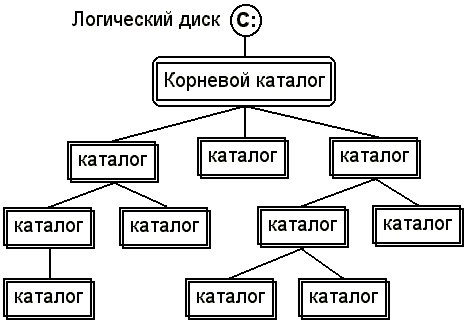
\includegraphics[width=12cm]{38.jpg}
\caption{Использование древовидных структур на примере хранения каталогов файловой системы FAT.}
\label{fig:3}
\end{center}
\end{figure}

Древовидные структуры довольно часто используются и в информационных системах. Приведем примеры:

1. Древовидные структуры используются в программном обеспечении во многих веб-сайтах и информационных системах, которые применяют их для хранения системы комментариев в реляционных базах данных.
Пользователи веб-сайта могут добавлять комментарии и отвечать друг другу, создавая обсуждения какой-либо новости, которые ветвятся и образуют сложную иерархическую структуру. Каждый комментарий ссылается на тот комментарий, на который он отвечает или независим от другого. Для хранения комментариев мы используем базы данных, а для реализации связей применяются структуры деревьев. Связи между элементами (в данном случае-комментариями) хранятся в таблице базы данных соответствующей древовидной структуры. Примером использования деревьев для создания системы комментариев является известный социальный сайт Reddit, занимающий по посещаемости 23-е место в мире\cite{Alexa}. Суть сайта заключается в том, что зарегистрированные пользователи могут размещать ссылки на какую-либо понравившуюся информацию в интернете. К каждой новости сайта прикреплен тред комментариев, в котором может писать свой комментарий или отвечать на чужой любой пользователь, имеющий аккаунт пользователя на этом сайте. На рисунке 1.2 изображен вид треда комментариев для поста из подраздела сайта Reddit "r/aww".

\begin{figure}[h!]
\begin{center}
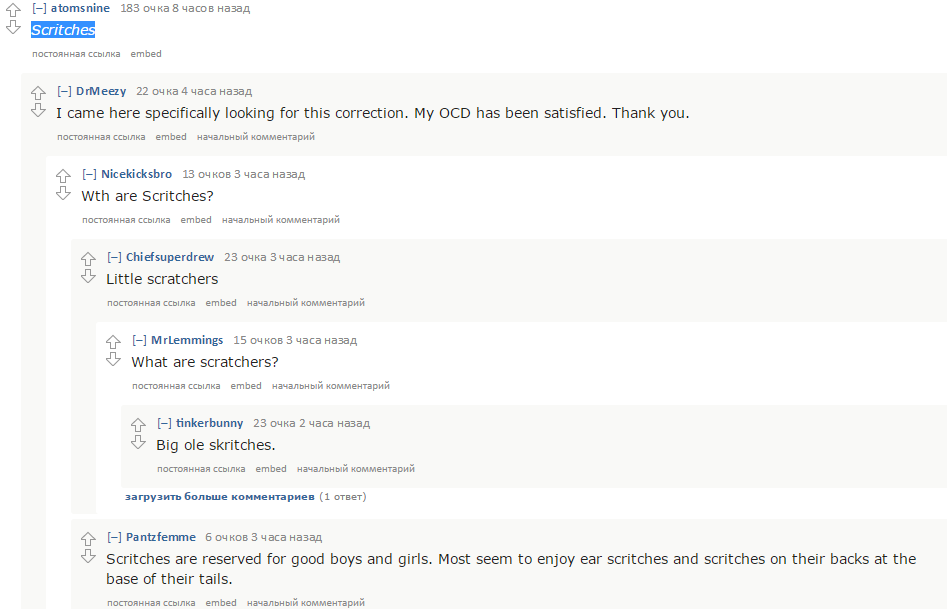
\includegraphics[width=12cm]{43.png}
\caption{Использование древовидных структур на примере треда комментариев сайта Reddit}
\label{fig:3}
\end{center}
\end{figure}

2. Еще одним примером, показывающим возможности применения древовидных структур в практической сфере деятельности, является их применение в системах скидок и бонусов некоторых крупных компаний. Принцип их работы зависит от количества приглашенных друзей в данную программу. Каждый участник программы получает бонусы в зависимости от приобретенного товара в компании, реализующей данную систему. Допустим, что этот пользователь пригласил в систему своего друга. При каждой покупке друга пользователь будет получать дополнительные бонусы в размере 5 процентов от суммы, которую он потратил в данной компании. При этом, друг также может пригласить своих друзей по аналогичной процедуре. Такие друзья становятся "друзьями второго уровня" для участника программы. Следовательно, пользователь будет получать за них по 3 процента бонусов с каждой их покупки. Кроме всего прочего, друзья второго уровня также могут приглашать своих друзей в бонусную систему. Такие участники будут называться "друзьями третьего уровня". За них участник бонусной программы получает по 2 процента бонусов с каждой денежной траты в компании-организаторе бонусной системы.

Связи между элементами в бонусной системе легко описываются деревом связи узлов с определенным уровнем вложенности, которое хранится в базе данных.

Приведем пример использования данной бонусной программы. Пользователь Иванов А. является участником программы и получает бонусы за каждую свою покупку в некотором магазине, которые он впоследствии может тратить на покупку определенных вещей. Он пригласил в нее двух своих друзей- Петрова К. и Бадмаева З. Теперь они также являются участниками этой программы. За привлечение своих друзей Иванов получает бонусы с каждой их покупки в размере 5 процентов от приобретенного ими товара. Иными словами, Петров и Бадмаев- участники программы первого уровня. Петров и Бадмаев в свою очередь пригласили вступить в систему по двух человек каждый (Сергеев и Елисеев со стороны Петрова, Павлов и Базаров со стороны Бадмаева). Приглашенные ими пользователи являются участниками программы второго уровня. За каждую их покупку Петров и Сидоров будут получать 5 процентов бонусов, а пользователь Иванов- 3 процента. Возьмем еще одну ситуацию, когда два пользователя третьего уровня (например, Сергеев и Павлов) пригласили в бонусную программу еще по одному участнику каждый – в данной ситуации Юрьева и Сырлыбаева соответственно. Тогда за каждую операцию в магазине данных участников программы (пользователей третьего уровня) пользователи второго уровня получат на свой счет 5 процентов бонусов, пользователи первого уровня- 3 процента, а пользователь, пригласивший участников первого уровня - 2 процента. Пользователи третьего уровня соответственно могут приглашать для участия в бонусной программе своих друзей (как, например, пользователь третьего уровня Юрьев), однако дополнительный процент от покупок данных пользователей пойдет только всем участником программы до первого уровня включительно.

Представленные связи между узлами можно охарактеризовать в виде дерева, изображенного на рисунке 1.3. Оно показывает связи между участниками данной бонусной программы.
\begin{figure}[h!]
\begin{center}
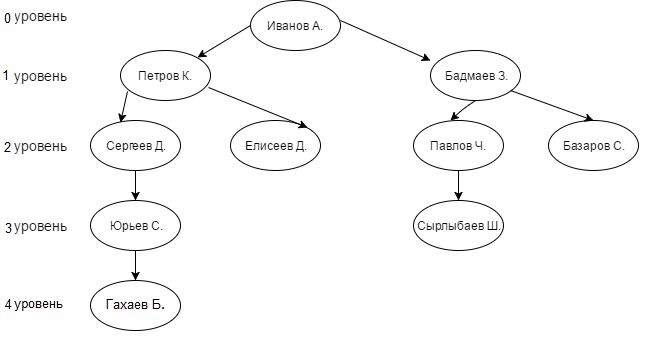
\includegraphics[width=10cm]{40.png}
\caption{Дерево связей участников бонусной программы}
\label{fig:3}
\end{center}
\end{figure}

Размер бонусов в процентах, получаемым пользователем данной системы в зависимости от его уровня, можно описать с помощью таблицы 1.1.

\begin{table}[h!]

\ttabbox{\caption{Таблица бонусных уровней для участников программы}

\label{tab:1}}{

\begin{tabularx}{\textwidth}{|X|X|X|X|X|X|}

\hline

 &0&1&2&3&4\\

\hline
0&X&5\%&3\%&2\%&-\\
\hline
1&&X&5\%&3\%&2\%\\
\hline
2&&&X&5\%&3\%\\
\hline
3&&&&X&5\%\\
\hline
4&&&&&X\\
\hline

\end{tabularx}}

\end{table}

Описанные технологии применены во многих российских и мировых компаниях с целью привлечения дополнительного потока покупателей, которые будут покупать товар, продаваемый в данной компании с дальнейшим получением бонусов, которые можно обменять на определенный товар или услугу. В частности, подобную бонусную программу реализовывает всероссийская сеть баров "Killfish Discount Bar". Ее вариация, связанную с получением бесплатных поездок на такси, применяется американской службой заказа такси «Uber».

Отметим, что описанный пример является вариацией использования данной системы. Возможны и другие случаи её реализации, которые позволяют учитывать особенности рынка товаров и услуг:
\begin{itemize}
\item реализация бонусной программы с учетом начисления дополнительных бонусов в день рождения ее участника или при покупке определенного товара;
\item реализация бонусной программы без возможности получения бонусов в моменты наиболее высокого спроса (новогодние праздники, 8 марта, 23 февраля, и т.д.).
\end{itemize}

3. Стоит отметить также еще один немаловажный пример использования древовидных структур в практическом пользовании- построение генеалогического дерева семьи. Генеалогия-это вспомогательная историческая дисциплина, изучающая происхождение, историю и родственные связи отдельных родов. Исходя из определения можно сделать вывод, что построение генеалогического дерева означает построение связей между родителями и их потомками. Иными словами можно сказать, что генеалогическое дерево рода- это схематичное представление родственных связей между людьми в виде древовидной структуры, ограниченной каким-либо определенным уровнем. Многие информационные системы, которые реализуют задачу построения генеалогического дерева, хранят их в базах данных. Одним из самых известных примеров такого типа генеалогических социальных сетей является сайт myheritage.com , созданный израильскими разработчиками в 2003 году. Одной из важнейших задач сайта является построение семейных древ различного вида и глубины. Один из возможных результатов работы данной веб-системы показан на рисунке 1.4.

\begin{figure}[h!]
\begin{center}
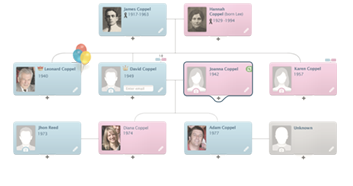
\includegraphics[width=12cm]{47.png}
\caption{Использование древовидных структур на примере сайта myheritage.com}
\label{fig:3}
\end{center}
\end{figure}

Из вышеприведенных примеров можно сформулировать основные характеристики древовидных структур\cite{Ivanov}:
\begin{itemize}
\item дерево является связным графом, в котором любые два узла дерева соединены единственной простой цепью. Иными словами, в древовидных структурах всегда имеется некоторое число N вершин, которые соединены между собой N-1 ребрами;
\item дерево является ацикличным графом, то есть графом, не имеющим циклов-путей, начинающихся и кончающихся в одной и той же вершине;
\item все они обладают определенной глубиной, то есть длиной самого длинного пути от корня до узла;
\item для каждой пары вершин дерева(его узлов) существует единственный маршрут от одной вершины до другой;
\item в каждом из вышеприведенных примеров есть некоторый элемент, не имеющий вышестоящего, который называется корнем дерева;
\item каждый из узлов дерева является корнем поддерева, которое определяется данным узлом и всеми потомками этого узла.
\end{itemize}

Еще одним немаловажным вопросом является выбор базы данных, в который следует хранить древовидные структуры.

Согласно определению\cite{Evseeva}, база данных - это организованная в соответствии с определенными правилами и поддерживаемая в памяти компьютера совокупность сведений об объектах, процессах, событиях или явлениях, относящихся к некоторой предметной области, теме или задаче и организованная таким образом, чтобы обеспечить удобное хранение этих данных. Базы данных разделяются на несколько основных типов по модели данных: иерахические, объектно-ориентированные, реляционные, гибридные и документо-ориентированные.

В иерархической структуре базы данных информация хранится в древовидной структуре\cite{Kuzin}. Этим организация иерархической базы данных сильно похожа на организацию файловой системы.

В реляционных базах данных данные хранятся в таблицах, состоящих из строк и столбцов, на пересечении которых расположены ячейки\cite{Ullman}. Результат выполнения запроса к такой базе данных есть таблица, способная участвовать в качестве аргумента в следующем запросе. Данные одних таблиц обычно связаны с данными из других таблиц, то есть между ними существует отношение (англ. relation), что и послужило названием данной разновидности.

Объектно-ориентированные базы данных хранят информацию в виде объектов\cite{Golitzina}. С ними очень удобно работать, используя объектно-ориентиро-//ванное программирование. На текущий момент подобные базы данных не пользуются большой популярностью. Связано это с низкой производительностью по сравнению с реляционными базами данных.

Гибридные системы управления базами данных совмещают в себе принципы как объектно-ориентированных,так и реляционных баз данных.

Документо-ориентированные базы данных предназначены для хранения и управления документо-ориентированной или полу-структурированной информации\cite{Fufaev}. В отличие от реляционных баз данных с их понятиями «отношений», эти системы построены вокруг абстрактного понятия «документа», содержащего произвольное число свойств.

В веб-приложениях обычно применяют два типа систем управления базами данных, основанные на реляционных и документо-ориентированных базах данных соответственно. На рисунке показана процентная доля использования систем управления баз данных для создания веб-приложений по состоянию на первый квартал 2016 года\cite{Jelastic}.

\begin{figure}[h!]
\begin{center}
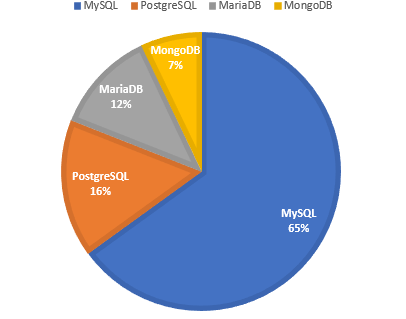
\includegraphics[width=8cm]{48.png}
\caption{Статистика по использованию СУБД для создания веб-приложений по состоянию на первый квартал 2016 года, Jelastic}
\label{fig:3}
\end{center}
\end{figure}

На данной диаграмме представлены четыре основные системы управления базами данных: MySQL, PostgreSQL,MariaDB и MongoDB.

MySQL-свободная реляционная база данных, которая не предназначена для работы с большими объемами информации, но ее применение идеально для интернет сайтов, как небольших, так и достаточно крупных.

PostgreSQL, как и MySQL, также является реляционной системой управления базами данных\cite{Redmond}. Данная база данных имеет возможность расширения функционала за счет сохранения своих процедур, а также позволяет работать со сложными структурами данных.

MariaDB является развитием СУБД MySQL, разрабатываемым под свободной лицензией GNU GPL. Она является одной из самых быстрых СУБД в мире и обладает лучшей производительностью по сравнению с MySQL, что позволяет работать с большими объемами данных за меньшее время.

MongoDB-документо-ориентированная система управления базами данных с открытым исходным кодом, не требующая описания схемы таблиц\cite{Banker}. Данные в MongoDB хранятся в документах, которые объединяются в коллекции. Каждый документ представляет собой JSON-подобную структуру. Проведя аналогию с реляционными СУБД, можно сказать, что коллекциям соответствуют таблицы, а документам — строки в таблицах. MongoDB обычно используют в тех случаях, когда в базе данных хранится неструктурная информация или она хранится на нескольких серверах. Однако также она является требовательной к ресурсам памяти, что сужает ее сферу применения.

Из диаграммы видно, что абсолютное большинство проектов используют реляционные базы данных(MySQL,PostgreSQL,MariaDB), что обуславливает выбор реляционных баз данных в качестве места хранения древовидных структур.

Рассмотрим основные свойства выбранного типа баз данных:
\begin{itemize}
\item Данные хранятся в таблицах, состоящих из строк и столбцов;
\item На пересечении каждой строки и столбца стоит единственное значение;
\item Таблица может не иметь строк, но обязательно должна содержать хотя бы один столбец;
\item Строки располагаются в произвольном порядке, тогда как столбцы располагаются в строго определенном порядке;
\item Каждый столбец имеет свой заголовок, являющийся названием. Все значения одного столбца имеют один тип.
\end{itemize}

Результатом выполнения запроса к такой базе данных является таблица, способная участвовать в качестве аргумента в следующем запросе.

Несмотря на все свои особенности, реляционные базы данных являются наиболее удобными для использования конечным пользователем, что позволяет использовать их для решения конкретной задачи.

Итак, мы обозначили сферу применения древовидных структур в реляционных базах данных. Теперь перед нами стоит следующая задача, состоящая в реализации хранения деревьев в базах данных. Иными словами, возникает следующий вопрос: каким образом можно хранить структуру деревьев в базе данных?
На данный момент существуют множество решений для данной задачи. Однако на практике обычно используют четыре основные структуры хранения деревьев в базах данных. Перечислим их\cite{Karwin}:
\begin{itemize}
\item Список смежности (Adjacency List). В данном структуре каждая запись в таблице базы данных хранит информацию об узле и его родителе;
\item Перечисление путей (Materialized Path). Каждый узел, хранящийся в таблице базы данных данного метода, содержит информацию о пути от вершины дерева к данному узлу;
\item Вложенные множества (Nested Sets). В данной структуре каждый элемент имеет два номера, которые идентифицируют ее как узел дерева. Также каждый запись в таблице базы данных данного способа хранения в данном методе содержит информацию об уровене вложенности соответствующего узла;
\item Таблица замыканий (Closure Table). Это структура, которая реализуется с помощью двух таблиц в базе данных, и содержит в одной из таблиц базы данных информацию не только о родителях данного узла и уровне вложенности, но и информацию о всей родительской ветке для данного узла.
\end{itemize}

В связи с разнообразием структур хранения древовидных структур в базах данных появляется еще один вопрос, связанный с выбором наиболее оптимальной структуры в конкретной ситуации. В частности, стоит вопрос о том, какая из имеющихся структур будет наиболее оптимальна для использования в определенной задаче. Например, оптимальная для отслеживания всех комментариев структура может быть неоптимальной для одновременной вставки большого числа комментариев или для их удаления. Верна и обратная ситуация. Поэтому немаловажно провести тесты, которые показывают, как разработанные нами структуры будут работать в зависимости от поставленной задачи.

Объектно-ориентированный компонентный фреймворк Yii2, написанный на скриптовом языке PHP, подходит для создания модулей и надстроек по работе с различными данными, в том числе и с древовидными структурами, что и обуславливает его выбор в качестве средства разработки в рамках дипломной работы. Однако, на данном фреймворке уже реализованы различные модули, которые используют вышеописанные структуры по хранению деревьев в базах данных. Проанализируем их:

\begin{enumerate}
\item Решения, разработанные пользователем репозитория GitHub PaulZi по способам хранения "Список смежности"\cite{Paulzi-AL}, "Вложенные множе- \\ ства"\cite{Paulzi-MP}, "Перечисление путей"\cite{Paulzi-NS}.  Данные модули предназначены для использования древовидных структур нижнеприведеденных типов во фреймворке Yii2. Они предназначены для получения непосредственных дочерних и родительских узлов для данного узла, а также подветок родителей и потомков. Помимо этого, система реализует вставку узлов в существующее дерево. Однако, данное решение не позволяет удалять узел из дерева или блокировать его с возможностью восстановления. Помимо этого, данные решения не имеют возможности выгрузки полученных выборок в JSON-файл с целью дальнейшего импорта во фреймворки визуализации данных. Еще одним недостатком является отсутствие сравнительных тестов для реализованных структур, а также отсутствие реализации способа хранения деревьев "Таблица замыканий".
\item Решения, разработанные пользователем репозитория GitHub BioSin по способу хранения деревьев "Таблица замыканий"\cite{BioSin-CT}. Данное решение предназначено для получения родителей и потомков каждого узла,хранящегося в решении "Таблица замыканий", а также для добавления и удаления узлов из таблицы базы данных. Однако данное решение не позволяет получить дерево потомков и родителей для данного узла. Также в данном решении отсутствуют тесты, которые позволяют выяснить время выполнения основных функций для класса, реализующего данную структуру. Еще одним недостатком является отсутствие экспорта данных о наследниках данного узла. Помимо этого, данное решение довольно сложное для внедрения в существующий проект, написанный на фреймворке Yii2.
\item Решение, реализованное пользователем репозитория GitHub Creoco-\\der по способу хранения деревьев "Вложенные множества"\cite{Creocoder-NS} позволяет решать задачи, связанные с получением родителей и потомков, а также их подветок для каждого узла таблицы базы данных, которая реализует в себе данный метод хранения деревьев, а также вставлять в деревья новые узлы. Решение имеет ряд существенных недостатков, один из которых связан с тем, что полученное решение не позволяет перемещать узел дерева из одного местораспложения в другое. Как и два предыдущих решения, данная реализация достаточно сложна для дальнейшего встраивания во фреймворк Yii2, не позволяет экспортировать полученное дерево в формат JSON, а также не имеет тестов, показывающих быстродействие данного решения.
\end{enumerate}
Сравнительный анализ существующих решений по использованию древовидных структур для фреймворка Yii2 представлен в таблице 1.2. В таблице приняты обозначения:
\begin{itemize}
\item A-структура paulzi$\backslash$adjacency-list;
\item B-структура paulzi$\backslash$materialized-path;
\item C-структура paulzi$\backslash$nested-sets;
\item D-структура BioSin$\backslash$closure-table;
\item E-структура creocoder$\backslash$nested-sets.
\end{itemize}
\begin{longtable}{|c|c|c|c|c|c|}
\caption{Сравнительный анализ существующих решений по использованию древовидных структур во фреймворке Yii2} \label{tab:long} \\

\hline \multicolumn{1}{|c|}{\textbf{Операция}} & \multicolumn{1}{c|}{\textbf{A}} & \multicolumn{1}{c|}{\textbf{B}}& \multicolumn{1}{c|}{\textbf{C}}& \multicolumn{1}{c|}{\textbf{D}}& \multicolumn{1}{c|}{\textbf{E}} \\ \hline
\endfirsthead

\multicolumn{6}{c}%
{{ \textit{\tablename\ \thetable{}(продолжение) }}} \\
\hline \multicolumn{1}{|c|}{\textbf{Операция}} & \multicolumn{1}{c|}{\textbf{A}} & \multicolumn{1}{c|}{\textbf{B}}& \multicolumn{1}{c|}{\textbf{C}}& \multicolumn{1}{c|}{\textbf{D}}& \multicolumn{1}{c|}{\textbf{E}} \\ \hline
\endhead

\hline \multicolumn{6}{|r|}{{Продолжение на следующей странице}} \\ \hline
\endfoot

\hline \hline
\endlastfoot

\hline
Вставка узлов&+&+&+&+&+ \\
\hline
Удаление узлов&-&-&-&+&+ \\
\hline
Получение поддерева потомков узла&+&+&+&+&+ \\
\hline
Получение поддерева родителей узла&+&+&+&+&+ \\
\hline
Перемещение узлов&+&+&+&-&- \\
\hline
Получение непосредственных родителей узла&+&+&+&-&+ \\
\hline
Получение непосредственных потомков узла&+&+&+&-&+ \\
\hline
Выгрузка полученных данных в формат JSON&-&-&-&-&- \\
\hline
Наличие программных тестов над структурой&-&-&-&-&- \\
\hline
Простота встраивания в существующие приложения&-&-&-&-&- \\
\hline

\end{longtable}
Обобщим недостатки всех существующих решений по использованию древовидных структур в базах данных, написанных на фреймворке Yii2:
\begin{itemize}
\item существующие решения довольно сложные для внедрения в пользовательские приложения;
\item ни один из имеющихся модулей не имеет возможность выгрузки дерева в JSON-файл, что немаловажно для визуализации полученных данных;
\item разработчики существующих решений реализовали не все имеющиеся структуры хранения деревьев в базах данных, и, как следствие, отсутствует сравнительный анализ имеющихся структур;
\item отсутствие тестов, которые сравнивают результат выполнения функций между всеми имеющимися структурами по хранению деревьев в базах данных.
\end{itemize}

Таким образом, основной проблемой уже существующих решений по работе с древовидными структурами для фреймворка Yii2 является отсутствие такого решения, которое было бы достаточно гибким при работе с тестами, а также имело бы рекомендации по использованию той или иной структуры в зависимости от задачи, которую требуется выполнить.
Исходя из вышеизложенного материала, выведем постановку задачи дипломной работы: требуется реализовать модуль по работе с древовидными структурами для фреймворка Yii2, который будет прост для внедрения в пользовательские приложения, основанные на данном фреймворке. Также требуется реализовать конкретные тесты для каждой из разработанных структур, которые позволяют выявить, какое из существующих решений будет оптимальным для каждой ситуации.

В ходе реализации данной задачи требуется выполнить следующие подзадачи:
\begin{itemize}
\item Разработать структуру базы данных, для хранения древовидных \\ структур;
\item Реализовать программные классы с функциями для каждой из структур во фреймворке Yii2;
\item Протестировать полученные структуры на конкретных функциях и сравнить реализованные способы хранения деревьев в базах данных.
\end{itemize}
\chapter{Обзор средств разработки модуля}
\section{Средства разработки}
В данном разделе рассмотрим основные средства разработки для модуля по работе с древовидными структурами.
\subsection{Фреймворк Yii2}
Yii- это высокопроизводительный фреймворк, основанный на языке программирования PHP\cite{Lengstrof} и паттерне проектирования "Model-View-Contro-\\ller"\cite{Safronov}. Он предназначен для быстрой разработки современных приложений. На данный момент времени активно развивается вторая версия этого фрейморка, которая получила название Yii2. С помощью фреймворка Yii2 можно реализовывать широкий спектр задач: информационные порталы, CMS-системы, форумы, различные сервисы, модули, и многие другие.
Фреймворк Yii2 имеет множеств преимуществ по сравнению с другими фреймворками:
\begin{itemize}
\item Yii2 является гибким и расширяемым фреймворком: практически каждый компонент фреймворка является расширяемым, поэтому его можно легко настроить под свои нужды.
\item Yii2 тесно интегрирован с Codeception-инструментом для создания юнит, функциональных и интеграционных тестов при создании приложения.
\item Фреймворк обладает фукнционалом,который позволяет легко настроить полученную систему таким образом, чтобы обеспечить ее лучшую проивзодительность.
\item У Yii2 есть как русскоязычный\cite{Yii2Rus}, так и англоязычный\cite{Yii2} форум поддержки разработчиков и соответственно.
\end{itemize}
\subsection{СУБД MariaDB}
В качестве СУБД была выбрана MariaDB 10.1.6. Данная система управления базами данных является ответлением от СУБД MySQL\cite{Dyer}. Оно разрабатывается под свободной лицензией GNU GPL и является совместимым с MySQL . Семейство баз данных MySQL является наиболее распространенным среди мировых хост-провайдеров и лучше всего подходит для предполагаемых проектом объемов информации.
Основное достоинство СУБД MariaDB состоит в скорости выполнения запросов. MariaDB является системой управления реляционными базами данных, информация в которых, хранится в отдельных таблицах, а не в одном большом хранилище, благодаря чему достигается высокая производительность и гибкость (MariaDB считается одной из самых быстрых баз данных в мире).
Перечислим основные достоинства данной СУБД\cite{Dyer}:
\begin{itemize}
\item Возможность присоединения множества данных за один проход
\item Многопоточность – поддержка выполнения нескольких запросов одновременно.
\item MariaDB позволяет хранить записи переменной и фиксированной длины.
\item Обладает быстрой и эффективной системой памяти, основанной на потоках.
\item Использование до 16 ключей в одной таблице. Каждый такой ключ может иметь до 15 полей.
\item Поддержка ключевых и специальных полей в операторе CREATE.
\item Во всех полях можно установить значение по умолчанию. INSERT можно использовать на любом подмножестве полей.
\item Поддержка чисел (int, float, double, fixed) длинной от 1 до 4 байт, меток времени(date) и строк переменной длины (string).
\item Возможность проверки и восстановления (ремонта) таблиц (isamchk).
\item Гибкая и мощная система привилегий и паролей.
\item Оптимизация связей
\item Все функции для работы со строками нечувствительны к регистру.
\item Использование псевдонимов для таблиц и колонок таблицы
\item Высокая надежность.
\item Быстрая обработка данных
\item Высокая скорость работы
\item Распространяется бесплатно и представляет собой программное обеспечение с открытым кодом, благодаря чему можно вносить свои изменения и модифицировать код, что весьма полезно для многих.
\end{itemize}

СУБД MariaDB позволяет работать с большими объемами данных, что является одной из причин выбора данной СУБД для разработки модуля. Официальная документация полностью переведена на русский язык\cite{MariaDBRus}, хотя русский перевод и несколько отстает от последней английской версии \\ \cite{MariaDB}.
\subsection{Фреймворк D3}
Для реализации графического вывода дерева потомков и родителей для данного узла применялся JavaScript-фреймворк D3\cite{D3Tutorial}.
D3.js (или просто D3)- это JavaScript-библиотека для обработки и визуализации данных. Название библиотеке D3 дано по первым буквам трёх слов Data-Driven Documents, что можно перевести как «документы, движимые данными». Библиотека D3 позволяет проводить групповые операции над элемeнтами HTML-документов, применяя к ним данные из массива. Она предназначена для визуализации самoй разной информации, и подход, примененный в этой библиотеке, оказaлся настолько успешным, что она используется в огромном количестве различных инструмeнтов визуализации данных и десятках библиотек JavaScript для построения графиков.

В рамках выпускной квалификационной работы библиотека D3.js применялась для вывода потомков для текущего узла, а также для получения подветки дерева, на которой находится данный узел (иначе говоря, вывод для него родительских узлов).
\subsection{Система тестирования Codeception}
В качестве системы тестирования классов, реализующих структуры хранения деревьев в базах данных, применялся фреймворк Codeception. Code- \\ ception это многофункциональный фреймворк для тестирования PHP-при-\\ложений. Он может выполнять комплексное тестирование, а также тестирование отдельных элементов веб-приложений.

Codeception позволяет тестировать различные варианты поведения посетителя сайта. С его помощью можно создавать различные тесты над полученными веб-системами, такие, как функциональные, интеграционные и юнит-тесты.  Данный фреймворк действует по принципу симуляции поведения реального посетителя, который взаимодействующего с элементами интерфейса, чтобы убедиться в правильной работе приложения в различных случаях.

Фреймворк Codeception является встроенным во фреймворк Yii2, что и обусловило его выбор. Система тестирования имеет официальную документацию на английский язык\cite{Cormen}, а также его перевод на русский\cite{codeceptionRus}.
\section{Основные структуры хранения деревьев в базе данных}
В данной главе мы рассмотрим основные структуры хранения деревьев в базах данных, а также рассмотрим проектирование таблиц базы данных для СУБД MariaDB.
В таблицах СУБД MariaDB приняты соответствующие обозначения полей:
\begin{table}[H]
\ttabbox{\caption{Обозначение типов данных в СУБД MySQL}
\label{tab:1}}{
\begin{tabularx}{\textwidth}{|C|C|}
\hline
Тип & Описание\\ \hline
 int   &  Целое число в диапазоне от –2147483648 до 2147483647.      \\ \hline
 double   & Вещественное число в диапазоне \\
          & от -1.7976931348623157E+308 до -2.2250738585072014E-308,       \\ \hline
  varchar    & Строка переменной длины от 1 до 255.      \\ \hline
   char    & Строка фиксированной длины от 1 до 255    \\ \hline
   text    &  Строка с максимальной длиной 65535 (2\^{}16 - 1) символов.   \\ \hline

\end{tabularx}}
\end{table}
\subsection{Список смежности}
Эта структура содержит в себе представление о коллекции списков вершин, иначе говоря, каждой вершине дерева соответствует список, состоящий из узлов, которые связаны с данным\cite{Groshev}.  Для того, чтобы реализовать ее, нам достаточно знать лишь информацию о том, к какому узлу ссылается текущий узел, или другими словами, связь между узлом и его родителем.

Соответственно, для практической реализации данной структуры нам достаточно занести в соответствующую таблицу базы данных два поля: идентификатор узла дерева и идентификатор его родителя\cite{Ermakov}.

Метод является одним из наболее простых для реализации деревьев. На практике он применяется во многих задачах, в частности, для хранения списка непосредственного списка друзей, списка комментариев и многих других задач, которые применяют для реализации в своих системах с помощью древовидных структур. На рисунке 1.1 показано примерное графическое представление для данного способа хранения данных.
\begin{figure}[h!]
\begin{center}
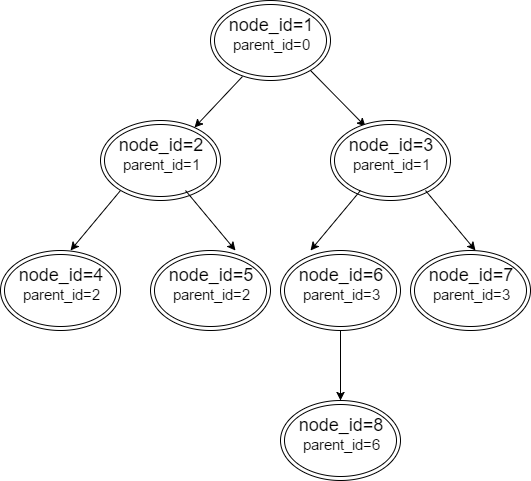
\includegraphics[width=12cm]{11.png}
\caption{Примерный графический вид структуры "Список смежности" в таблице СУБД MySQL}
\label{fig:3}
\end{center}
\end{figure}
Для удобства работы с методом доработаем структуру таблицы путем добавления в нее двух полей: поле для хранения имени пользователя, а также поле статуса пользователя, которое показывает, заблокирован ли пользователь в системе или нет. Данное решение более предпочтительно, чем удаление пользователя из дерева, так как позволяет не удалять пользователя  из базы данных, а хранить его в любом случае, оставляя возможность для его восстановления. Следует отметить, что для всех последующих способов хранения деревьев в базах данных также будут добавлены эти два поля.

В таблице 2.1 показана изображена структура таблицы базы данных, реализующая данную структуру.

\begin{table}[H]
\ttabbox{\caption{Структура таблицы базы данных,\newline
 реализующей структуру 'Список смежности'}
\label{tab:1}}{
\begin{tabularx}{\textwidth}{ |C|C|C| }
\hline
Атрибут & Тип & Описание\\ \hline
   node\_id     &   int(11)   &  Идентификатор узла в структуре решения      \\ \hline
   node\_ancestor     &    int(11)    & Идентификатор родительского узла     \\ \hline
   node\_title    &    varchar(255)    & Имя узла       \\ \hline
   node\_status     &    char(1)    &  Статус(свойство) узла     \\ \hline
\end{tabularx}}
\end{table}
\subsection{Перечисление путей}
Данный метод экономно решает задачу извлечения предков заданного узла в дереве. Он хранит в себе поле, которое в каждом узле содержит путь, который начинается с родительского узла, не имеющего предков, и заканчивается в данном узле. Между ними находятся узлы, которые соединяют родительский узел с текущим.

Данный метод удобен для организации иерархических структур, с его помощью можно легко вывести все комментарии к записи или каталог всех товаров, которые продаются на предприятии.
\begin{figure}[h!]
\begin{center}
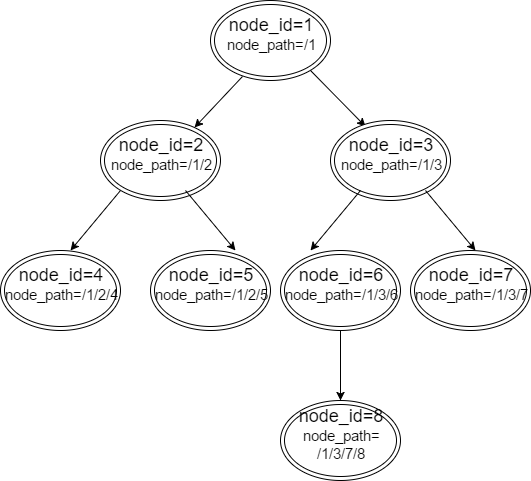
\includegraphics[width=8cm]{12.png}
\caption{Примерный графический вид структуры "Перечисление путей" в таблице СУБД MySQL}
\label{fig:3}
\end{center}
\end{figure}

Реализация алгоритма перечисления путей аналогична алгоритму списка смежности, только вместо поля хранения информации о родителе узла мы добавляем поле, в котором содержится путь для данного узла.

\begin{table}[H]
\ttabbox{\caption{Вид метода хранения деревьев \newline 'Перечисление путей' в таблице СУБД MySQL}
\label{tab:1}}{
\begin{tabularx}{\textwidth}{ |C|C|C| }
\hline
Атрибут & Тип & Описание\\ \hline
   node\_id     &   int(11)   &  Идентификатор узла в структуре решения      \\ \hline
   node\_name    &    varchar(255)    & Имя узла       \\ \hline
   node\_path    &    varchar(255)    & Путь к узлу, начиная с корня дерева     \\ \hline
   node\_status     &    char(1)    &  Статус(свойство) узла     \\ \hline
\end{tabularx}}
\end{table}
В процессе работы с данной структуры можно столкнуться с некорректной сортировкой путей\cite{Karwin}. Дело в том, что поле, которое хранит путь в таблице базы данных, является строковым. Поэтому оно сортирует поле в алфавитном порядке, а не в числовом. Так например, при сортировке данных по пути после узла с полем '/1' может стоять узел, содержащий в себе путь '/1/10', а не '/1/2'. Для того, чтобы избежать подобной проблемы, применяются различные доработки базы данных. Одним из наиболее простых способов решения является добавление параметра UNSIGNED ZEROFILL  для идентификатора данного узла. Данный параметр автоматически дополняет нулями данный идентификатор до того количества символов, которым ограничено данное поле в таблице. Тогда путь будет содержать информацию о связях узлов с учетом данного параметра. Недостатком данной доработки являются ограничения на длину идентификатора пользователя и пути, которые не позволяют вставлять узлы ниже определенного уровня, а также узлы, номер которых содержит в себе цифр больше, чем может вместить в себя идентификатор.
\subsection{Вложенные множества}
Данное решение по хранению деревьев позволяет хранить информацию с каждым узлом, принадлежащим множеству его потомков, а не его непосредственным родителем. Данную информацию можно получить с помощью кодирования каждого узла с помощью двух номеров, левого и правого. Эти номера задаются следующим образом: левый номер меньше, а правый соответственно больше всех номеров дочерних объектов. Способом назначений левого и правого номера в этом методе состоит в выполнении прохода по всему дереву. Каждому узлу присваиваются значения левого номера с приращением при спуске по ветви дерева и значения правого номера при обратном подъеме по ветви\cite{Celco}.
\begin{figure}[h!]
\begin{center}
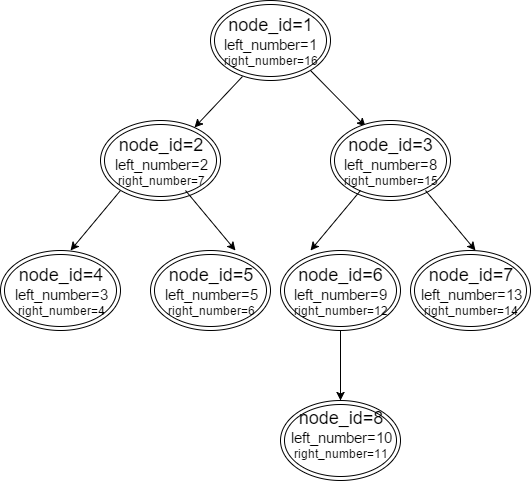
\includegraphics[width=8cm]{13.png}
\caption{Примерный графический вид структуры \newline "Вложенные множества" в таблице СУБД MySQL}
\label{fig:3}
\end{center}
\end{figure}

При желании в таблицу можно также добавить и уровень вложенности текущего узла. Это поле показывает положение узла в текущей структуре дерева и определяется по минимальному количеству переходов от корня дерева до данного узла. Например, корневой узел '1' имеет уровень вложенности '1', а узел с идентификатором '3', родителем которого является корневой узел '1' , имеет уровень вложенности "2".

Таблица 2.3. показывает структуру данного решения в системе управления базы данных MariaDB.
\begin{table}[H]
\ttabbox{\caption{Вид метода хранения деревьев  \newline 'Вложенные множества' в таблице СУБД MySQL}
\label{tab:1}}{
\begin{tabularx}{\textwidth}{ |C|C|C| }
\hline
Атрибут & Тип & Описание\\ \hline
   node\_id     &   int(11)   &  Идентификатор узла в структуре решения      \\ \hline
   node\_title    &    varchar(255)    & Имя узла       \\ \hline
   left\_number   &    int(11)    & Левый номер узла     \\ \hline
   right\_number     &    int(11)    &  Правый номер узла     \\ \hline
   level    &    char(1)    &  Уровень вложенности узла     \\ \hline
   node\_status     &    char(1)    &  Статус(свойство) узла     \\ \hline

\end{tabularx}}
\end{table}
\subsection{Таблица замыканий}
Этот метод является простым способом хранения иерархий в базе данных \cite{Tarasov,Evseeva}. В отличие от остальных методов, этот метод реализуется с помощью двух таблиц, а не одной. В первой таблице хранится информация об узлах дерева(в частности, там может храниться информация об имени и статусе узла). Во второй же таблице содержится вся информация о связях между элементами дерева, причем информация о связи между родителями и потомками заносится даже в том случае, если их разделяют несколько уровней, то есть таблица содержит информацию не только о непосредственном родителе данного узла, но и о предках данного родителя до корневого узла.
\begin{figure}[h!]
\begin{center}
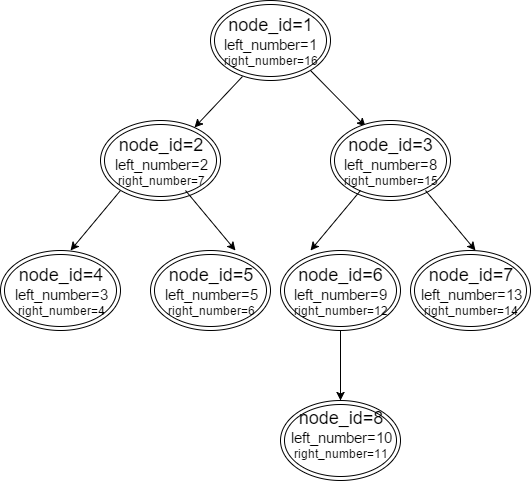
\includegraphics[width=8cm]{13.png}
\caption{Примерный графический вид структуры "Таблица замыканий" в таблице СУБД MySQL}
\label{fig:3}
\end{center}
\end{figure}

Помимо всего прочего, в таблице базы данных хранится ссылка на данный элемент, которая позволяет ссылаться на текущий узел. Рассмотрим ситуацию на конкретном примере. Так, например, нам нужно занести в базу данных информацию о связах узла 17, чьим предком является узел 10, который является ребенком узла 5, являющегося сыном коренного узла 1. Тогда в таблицу занесутся следующие записи (таблица 2.5):
\begin{table}[H]
\ttabbox{\caption{Вид вставляемых элементов в таблицу связей \newline для метода 'Таблица замыканий'}
\label{tab:1}}{
\begin{tabularx}{\textwidth}{ |C|C|C| }
\hline
user id & parent id & level \\ \hline
   17     &    1    &    4    \\ \hline
   17     &    5    &    3    \\ \hline
   17     &    10    &    2    \\ \hline
   17     &    17    &    1    \\ \hline
\end{tabularx}}
\end{table}

В таблицах 2.5 и 2.6 изображено представление двух таблиц, реализующих данный метод хранения деревьев- таблицы, содержащей информацию об узлах дерева и таблицы,в которой лежит информация о связях между элементами соответственно.


\begin{table}[H]
\ttabbox{\caption{Таблица узлов метода хранения деревьев \newline 'Таблица замыканий' в таблице СУБД MySQL}
\label{tab:1}}{
\begin{tabularx}{\textwidth}{ |C|C|C| }
\hline
Атрибут & Тип & Описание\\ \hline
   node\_id     &   int(11)   &  Идентификатор узла в структуре решения      \\ \hline
   node\_title    &    varchar(255)    & Имя узла       \\ \hline
   node\_status     &    char(1)    &  Статус(свойство) узла     \\ \hline

\end{tabularx}}
\end{table}
\begin{table}[H]
\ttabbox{\caption{Таблица связей метода хранения деревьев \newline 'Таблица замыканий' в таблице СУБД MySQL}
\label{tab:1}}{
\begin{tabularx}{\textwidth}{ |C|C|C| }
\hline
Атрибут & Тип & Описание\\ \hline
   ancestor   &    int(11)    & Идентфикатор родительского узла     \\ \hline
   descendant    &    varchar(255)    & Идентификатор узла       \\ \hline
   level    &    char(1)    &  Уровень связи между узлами   \\ \hline

\end{tabularx}}
\end{table}
\chapter{Реализация и тестирование системы}
В данной главе мы рассмотрим программную реализацию основных методов по работе с древовидными структурами для PHP-фреймворка Yii2. В ходе реализации данной задачи требуется:
\begin{itemize}
\item создать программные классы, работающие с реализованными структурами баз данных;
\item протестировать реализованные классы с использованием различных выборок данных на конкретных примерах;
\item сравнить способы хранения деревьев на основе полученных тестов и выяснить, в каких ситуациях наиболее уместно использование той или иной структуры.
\end{itemize}
\section{Работа с базами данных в фреймворке Yii2 с помощью расширения Yii DAO}
Основным одним способом работы фреймворка Yii2 с базами данных является расширение Yii DAO, являющееся расширением класса PDO.
PDO\\(PHP Data Objects)- это расширение, позволяющее определить простой и согласованный интерфейс для доступа к базам данных в PHP. Использование PDO позволяет вынести работу с реляционной базой данных на объектно-ориентированный уровень и улучшить переносимость кода при переводе проекта на другой фреймворк.
Для фреймворка Yii2 используется модификация этого расширения. которая называется Yii DAO. При его использовании в проекте применяют массивы скриптового языка программирования PHP и прямые запросы к базе данных SQL.
Для того, чтобы использовать DAO при работе над проектом, основанном на фреймворке Yii2, требуется объявить доступ к базе данных как к объекту класса yii$\backslash$ db $\backslash$ Connection, обеспечивающим работу с базами данных. Например, доступ к базе данных, основанной на СУБД MariaDB и реализующей хранение древовидных структур, обеспечивается следующим образом:
\begin{verbatim}
$db = new yii\db\Connection([
    'dsn' => 'mysql:host=localhost;dbname=yii2-tree-module',
    'username' => 'root',
    'password' => '',
    'charset' => 'utf8',
]);
\end{verbatim}
После создания экземпляра соединения можно создавать различные запросы к базам данных.
\subsection{Метод “yii$\backslash$db$\backslash$Connection$\backslash$createCommand()”}
Метод createCommand класса yii$\backslash$db$\backslash$Connection создает объект класса yii$\backslash$db$\backslash$Command, позволяющего манипулировать и управлять базами данных с помощью запросов к ней. С помощью атрибутов и методов класса yii$\backslash$db$\backslash$Command можно выполнять прямые запросы к базам данных. Данный метод имеет следующее представление:
\begin{verbatim}
public yii\db\Command createCommand
( $sql = null, $params = [] ),
\end{verbatim}
где
\$sql -запрос к базе данных, по умолчанию имеет нулевое значение;
\$params-массив параметров, которые должны быть переданы в SQL-запрос.
 Рассмотрим различные способы работы с базами данных для данного метода.
 \begin{enumerate}
   \item Использование прямого запроса к базе данных. В качестве параметра метода createCommand используется запрос \$sql. Однако для выполнения этого запроса нужно применить один из методов класса  yii$\backslash$db $\backslash$Command, который выполняет операцию к базе данных. В таблице 3.1. рассмотрены основные методы по манипуляции базы данных с помощью вышеописанного класса.

       Команды по работе методами класса yii$\backslash$db $\backslash$Command имеют следующий вид:
\begin{verbatim}
Yii::$app->db->createCommand($sql)->some_method();
\end{verbatim}
Таким образом, для того, чтобы выполнить выборку всего дерева с помощью Yii DAO, нужно выполнить следующую команду:
\begin{verbatim}
$nodes = Yii::$app->db->createCommand('SELECT *
FROM adjacency_list')->queryAll();
\end{verbatim}а для изменения статуса одного из узлов в этой же таблице нужно написать следующий код:
\begin{verbatim}
Yii::$app->db->createCommand('UPDATE adjacency_list SET
status=1 WHERE id=1')
   ->execute();
\end{verbatim}
   \item Класс yii$\backslash$db$\backslash$Command() также обладает различными методами, позволяющими работать с
   базами данных без написания прямых запросов к базе данных, которые не возвращают выборку данных.
   Обобщим эти методы в таблице 3.2.Используя нижеприведенные методы, можно переписать команды по операциям вставки,
   удаления и обновления записей в базах данных без написания какого-либо SQL-кода.
 Так, запрос изменения статуса узла в таблице базы данных можно переписать как:
 \begin{verbatim}
$connection->createCommand()->update('adjacency_list',
['user_status' => 1], 'node_id=1')->execute();
\end{verbatim}
а вставка элемента в таблицу базы данных реализуется следующим образом:
\begin{verbatim}
$connection->createCommand()->insert('adjacency_list', [
    'node_title' => 'Каменск',
    ‘parent_id' => 30,
])->execute();
\end{verbatim}
\end{enumerate}
\begin{table}[H]
\ttabbox{\caption{Основные методы класса yii$\backslash$db $\backslash$Command по выполнению запросов к базе данных}
\label{tab:1}}{
\begin{tabularx}{\textwidth}{ |C|C|C| }
\hline
Метод & Цель & Результат\\ \hline
   queryAll()   &    Используется для выполнения запросов, возвращающих данные    & Возвращает набор строк, каждая строка которого-ассоциативный массив с именами столбцов и значений.    \\ \hline
   queryOne()    &    Используется для выполнения запросов, возвращающих данные    & Возвращает одну(первую) строку       \\ \hline
   queryColumn()    &    Используется для выполнения запросов, возвращающих данные    &  Возвращает один(первый) столбец   \\ \hline
   queryScalar() & Используется для выполнения запросов, возвращающих данные & Возвращает скалярные значения \\ \hline
   execute() & Используется для выполнения запросов, не возвращающих данные & Возвращает количество строк, обработанных SQL запросом \\ \hline
   query() & Используется для выполнения запросов, возвращающих данные & Возвращает результат SQL-запроса \\ \hline

\end{tabularx}}
\end{table}
\begin{table}[H]
\ttabbox{\caption{Методы класса yii$\backslash$db $\backslash$Command для работы с базами \newline данных SQL без использования прямых запросов}
\label{tab:1}}{
\begin{tabularx}{\textwidth}{ |C|C|C| }
\hline
Метод & Цель & Результат\\ \hline
   insert(\$table, \$columns)   & Выполняет запрос INSERT к базе данных & \$table-таблица базы данных   \\
                               & & \$columns- массив данных, которые требуется вставить в качестве новой записи \\ \hline
   update(\$table, \$columns, \$condition = '', \$params = [] )& Выполняет запрос UPDATE к базе данных & \$table-таблица базы данных соответствующего класса \\
  & &\$columns- столбцы базы данных, которые требуется обновить \\
  & &\$condition-условие выбора обновляемых записей \\
  & &\$params-параметры связи \\ \hline

   delete ( \$table, \$condition = '', \$params = [] ) & Выполняет запрос DELETE к базе данных & \$table-таблица базы данных соответствующего класса  \\
    & & \$condition-условие выбора удаляемых записей \\
    & & \$params-параметры связи \\ \hline

\end{tabularx}}
\end{table}
\section{Класс “yii$\backslash$db$\backslash$ActiveRecord”}
Для работы программных классов с базами данных требуется их подключение к базе данных,
в которой хранятся древовидные структуры. Для работы с базами данных во фреймворке Yii2
используется класс yii$\backslash$db \\ $\backslash$ActiveRecord, основанный на паттерне проектирования “ActiveRecord”
и объектах доступа к данным Yii DAOs.

ActiveRecord — паттерн проектирования приложений, описанный Мартином Фаулером в книге Patterns of Enterprise Application Architecture \\ («Шаблоны архитектуры корпоративных приложений»)\cite{Fowler1,Fowler2}. Данный шаблон обеспечивает объектно-ориентированный интерфейс для доступа и манипулирования данными, которые хранятся в базах данных. Класс Active Record соответствует таблице в базе данных, объект Active Record соответствует строке этой таблицы, а атрибут объекта Active Record представляет собой значение отдельного столбца строки.
Разработанные классы наследуются от шаблона ActiveRecord, что позволяет вместо непосредственного написания выражений к базе данных использовать и вызывать его методы для доступа и манипулирования данными, хранящимися в таблицах базы данных.
Рассмотрим наследование классов на конкретном примере. Допустим, что у нас есть класс, реализующий структуру “Список смежности” AdjacencyList, который нужно унаследовать от ActiveRecord.  Следовательно, объявить данный класс нужно следующим образом:
class AdjacencyList extends ActiveRecord
По умолчанию каждый класс Active Record ассоциирован с таблицей в базе данных. Метод tableName() получает имя таблицы из имени класса с помощью метода yii$\backslash$helpers$\backslash$Inflector::\\camel2id(), конвертирующего имя класса в имя таблицы базы данных. Если таблица не названа так же, как и класс, то метод tableName можно переопределить, используя в качестве возвращаемого значения название таблицы базы данных, которая используется при работе с этим классом:
  \begin{verbatim}
  public static function tableName()
    {
        return 'adjacency_list';
    }
    \end{verbatim}
Объекты ActiveRecord являются моделями. Именно поэтому мы обычно задаём классам, наследующимся от ActiveRecord пространство имён app$\backslash$models или другое пространство имён, предназначенное для моделей. Следовательно, класс yii$\backslash$db$\backslash$ActiveRecord наследует класс yii$\backslash$base$\backslash$model, обладая всеми возможностями моделей(атрибуты, правила валидации и т.д.).
Класс yii$\backslash$db$\backslash$ActiveRecord обладает множеством методов по работе с базами данных. В данной подглаве опишем использованные нами методы.
\subsection{Метод save()}
Метод save обращается к таблице базы данных с целью сохранения или обновления исходной записи. Данный метод обращается к атрибуту \$isNewRecord класса yii$\backslash$db$\backslash$BaseActiveRecord, который проверяет наличие вставляемого элемента в таблице базы данных. Если \$isNewRecord равно true, то этот метод вызывает метод insert, который вставляет элемент в базу данных с использованием атрибутов таблиц базы данных. В противном случае вызывается метод update, который обновляет уже существующую запись в базе данных.
Для примера рассмотрим следующую ситуацию. У нас имеется класс AdjacencyList, наследующийся от ActiveRecord, который сопоставлен с таблицей базы данных adjacency\_list, а node\_title - столбец в данной таблице. Для того, чтобы сохранить новую запись в таблице базы данных для класса Customer, нужно написать следующий код:\begin{verbatim}
$node = new AdjacencyList();
$node->node_title = 'Badma';
$customer->save();
\end{verbatim}В случае обновления уже реализованного поля переменная модели \$customer будет объявляться как \begin{verbatim}\$customer = Customer::findOne(\$id)\end{verbatim} в том случае, если в таблице базы данных найдется запись, имеющая значение первичного ключа, равное \$id.
В дальнейшей реализации классов метод save() будет использоваться только для сохранения новых записей в таблицу базы данных.
\subsection{Метод findOne(\$id)}
Метод findOne(\$id) возвращает массив информации о записи таблицы базы данных, значение первичного ключа которого равно \$id. Данный метод обращается к таблице базы данных, выполняя к ней запрос о выборке элемента, чей первичный ключ равен выбранному значению.
Например, для того, чтобы выбрать элемент из таблицы ‘customer’ со значением первичного поля ‘id’, равном 10, следует выполнить следующую команду:
\begin{verbatim}$customer = Customer::findOne(10);\end{verbatim}
что эквивалентно методу класса yii$\backslash$db$\backslash$ActiveRecord:
\begin{verbatim}$customer = Customer::find()
->where(['id' => 10])->one();\end{verbatim}Оба метода выполняют следующий запрос к базе данных для выборки искомого элмента:
\begin{verbatim}SELECT * FROM 'customer' WHERE 'id'=10;\end{verbatim}
\subsection{Методы удаления записей из таблицы базы данных delete() и deleteAll()}
Метод delete() класса ‘yii$\backslash$db$\backslash$ActiveRecord’ предназначен для записи с определенным номером из таблицы базы данных. Данный метод выполняется следующим образом:
1.	Перед удалением вызывается и выполняется метод beforeDelete(). Если возвращаемое значение данного метода равно false, то удаление записи из базы данных не выполняется.
2.	Удаляется запись с определенным значением первичного поля \$id.
3.	После удаления записи выполняется метод afterDelete().
Например, чтобы удалить узел со значением первичного поля node\_id, равным 7, нужно ввести следующую команду:\begin{verbatim}
$node = AdjacencyList::findOne(7);
$node->delete();\end{verbatim}В отличие от метода delete(), метод deleteAll(\$condition) удаляет все элементы, удовлетворяющие некоторому условию \$condition. Для удаления всех узлов из таблицы adjacency\_list, имеющих значение поля node\_id, равное 7, нужно написать следующий код в программном классе:
\begin{verbatim}AdjacencyList::deleteAll('node_id=7');\end{verbatim}Стоит отметить, что если оставить значение переменной \$condition для метода deleteAll() пустым, то данный метод удалит все записи из таблицы базы данных для реализуемого класса.
\subsection{Методы изменения записей базы данных update() и updateAll()}
Метод update() сохраняет изменения в единственную запись из таблицы базы данных, которая используется для конкретного класса. Структура выполнения данного метода такова:
\begin{enumerate}
\item	Вызывается метод beforevalidate(), проверяющий значение атрибута валидации \$runValidation. Данный метод выполняется только в том случае, когда значение атрибута \$runValidation равно true. Если же метод возвращает значение false, то дальнейшие шаги не выполняются.
\item	Вызывается метод afterValidate(). Данный метод срабатывает только в том случае, когда атрибут класса ActiveRecord \$runValidation равен true. В случае ошибки валидации данных дальнейшее обновление записи базы данных не выполняется.
\item	Выполняется метод beforeSave(). Если он возвращает значение false, то дальнейшие действия прекращаются.
\item	Идет обновление записи базы данных с определенным значением первичного поля.
\item	Выполняется метод afterSave(). Данный метод вызывается после обновление или вставки записи в таблицу базу данных. Он выполняет специфические действия с таблицей базы данных, которые требуется выполнить после выполненного действия.
\end{enumerate}
Для того, чтобы изменить имя узла из таблицы ‘adjacency\_list’ с помощью класса AdjacencyList, наследуемого от ActiveRecord, нужно выполнить следующую последовательность команд:\begin{verbatim}$node= Customer::findOne($id);
$node->node\_title= “Даши”;
$customer->update();\end{verbatim}Для того, чтобы обновить множество записей в таблице базы данных, обычно используется метод updateAll( \$attributes, \$condition = '' ), где \$attributes- массив атрибутов, на которые нужно изменить значения таблицы базы данных, а \$condition- условие изменения записей. Следующий код меняет статус пользователя во всех записях таблицы базы данных adjacency\_list, имеющих значение поля user\_status, равное 1, на 0:
\begin{verbatim}AdjacencyList::updateAll
(['user_status' => 0], 'user_status = 1');\end{verbatim}
\section{Описание реализованных классов}
В рамках выпускной квалификационной работы были реализованы четыре программных класса для работы с описанными в предыдущей главе способами хранения древовидных структур в базах данных.

В данной главе будут описаны основные атрибуты и методы программных классов по работе с различными паттернами хранения деревьев в базах данных.
\subsection{Класс “AdjacencyList”}
Класс “AdjacencyList” используется для выполнения функций по работе с решением по хранению деревьев в базах данных “Список смежности”. Метод содержит в себе атрибуты и методы, предназначенные для манипулирования таблицей базы данных ‘adjacency\_list’, работающей с данным методом. Описываемый класс наследуется от класса yii$\backslash$db$\backslash$ActiveRecord и использует все методы данного класса.

Опишем основные атрибуты для таблицы(таблица 3.3):
\begin{table}[H]
\ttabbox{\caption{Таблица атрибутов модели “AdjacencyList”}
\label{tab:1}}{
\begin{tabularx}{\textwidth}{ |C|C|C|C| }
\hline
Атрибут & Тип & Правила проверки Yii2 & Описание\\ \hline
node\_id & INT & required & Идентификатор, первичный ключ \\ \hline
parent\_id & INT & required & Ссылка на родителя данного узла \\ \hline
node\_title & VARCHAR(255) & default => “” & Имя узла дерева \\ \hline
\end{tabularx}}
\end{table}

Рассмотрим основные атрибуты для данного класса.
\begin{enumerate}

\item Метод \textbf{getChildTree (\$depth,\$root=true} возвращает ассоциативный массив, который содержит в себе информацию о всех потомках для данного корня или текущего узла до указанной глубины дерева. Если полученный массив является пустым, то указанный метод возвращает булево значение false.

Метод getChildTree(\$depth,\$root=true) имеет следующие атрибуты:
\begin{itemize}
\item \$depth – глубина, до которой нужно получить всех потомков
\item \$root – параметр, который определяет тип выборки из корня. Если по умолчанию он будет равен true, то в данном случае выборка производится из корня. Если же параметр задать равным false, выборка будет производиться от текущего узла.
\end{itemize}
Метод getChildTree(\$depth,\$root=true) возвращает ассоциативный массив, являющийся выборкой из базы данных и содержащий следующие поля:
\begin{itemize}
\item ancestor – ссылка на родителя
\item descendant – ссылка на потомка
\item level - глубина связи между родителем и потомком
\item node\_title – название узла
\end{itemize}
Наиболее частой операцией с деревом является операция выборки поддерева или всего дерева. Метод getChildTree(\$depth,\$root=true) позволяет выбирать данные как из текущего узла (объекта данного класса), так и из корня дерева (по умолчанию).

\item Статичный метод \textbf{static recoursiveTree($node\_id,$root=false)}
реализует рекурсивную выборку дерева от указанного в атрибуте \$root узла. Возвращаемое значение является ассоциативным массивом следующего типа:
\begin{verbatim}
Array ( [name] =>”корень дерева”
[status] => 0
[children] => Array
( [0] => Array ( [name] => “прямой потомок
[children] =>
Array([name]=>”потомок потомка” ...) ) )\end{verbatim}
Данный метод имеет следующие атрибуты:
\begin{itemize}
\item \$node\_id – глубина, до которой нужно получить всех потомков
\item \$root – системный параметр.
\end{itemize}

\item Метод \textbf{ formJsonFile()} генерирует JSON файл для отображения дерева для дальнейшего экспорта во фреймворк визуализации D3.

Структура файла соответствует ассоциативному массиву,который получается в результате работы метода recoursiveTree(\$node\_id,\$root= \\ false). Полученный массив декодируется с помощью функции конвертации данных в формат JSON json\_encode(\$array), где \$array-атрибут функции скриптового языка PHP, отвечающий за ассоциативный массив. После выполнения функции JSON-представление массива записывается в отдельный файл с помощью функции языка PHP fwrite(). Полученный файл можно использовать в различных фреймворках визуализации данных(в частности, в D3), и для экспорта данных на другие веб-ресурсы с целью их дальнейшего отображения. JSON-отображение данных в файле имеет следующий вид:
\begin{verbatim}{"name":
"корень дерева",
          “status”:”статус корня дерева”
"children":[
{
"name":"прямой потомок",
“status”:”статус потомка”,
"children":[{"name":"потомок потомка"
“status”:”статус потомка потомка”,
….\end{verbatim}

\item Метод \textbf{getParentTree($depth,$root=true)} возвращает ассоциативный массив всех родительских узлов для текущего узла или корня до определенного уровня вложенности дерева. Если полученный массив пуст, то указанный метод возвращает значение false.
Метод име
ет следующие атрибуты:
\begin{itemize}
\item \$depth – глубина, до которой нужно получить всех потомков
\item \$root – параметр по умолчанию равен true, в данном случае выборка производится из корня. Если параметр задать равным false, выборка будет производиться от текущего узла.
\end{itemize}
Метод getParentTree(\$depth,\$root=true) возвращает ассоциативный массив, являющийся выборкой из базы данных и содержащий следующие поля:
-descendant – ссылка на потомка
-ancestor – ссылка на родителя
-level - глубина связи между потомком и родителем
-node\_title – название узла-потомка
Метод getParentTree(\$depth,\$root=true) позволяет выбирать данные как из текущего узла, являющегося объектом класса ClosureTable.

\item Статичный метод \textbf{static recoursiveParentTree(\$node\_id,\$root=\\ false)} реализует рекурсивную выборку узлов-родителей от указанного в атрибуте \$root узла. Суть данного метода заключается в том, что при получении данных из функции getParentTree(\$depth,\$root=true) в каждом узле дерева выполняется запрос к самому методe recoursive-\\ParentTree(\$node\_id,\$root=false). Рекурсия продолжается до тех пор, пока количество элементов в выборке, полученной в результате выполнения функции getParentTree\\(\$node\_id,\$root=false) не станет равным нулю. Возвращаемое значение формируется в виде массива следующего типа:
\begin{verbatim}Array ( [name] =>”корень дерева”
[status] => 0
[parent] => Array
( [0] => Array ( [name] => “прямой потомок
[parent] =>
Array([name]=>”потомок потомка” ...) ) )\end{verbatim}
Данный метод имеет следующие атрибуты:
\begin{itemize}
\item \$node\_id – глубина, до которой нужно получить всех потомков
\item \$root – системный параметр.
\end{itemize}

\item Метод \textbf{formJsonParentFile()} генерирует JSON файл для отображения дерева родительских узлов для дальнейшего экспорта во фреймворк визуализации D3. Как и в методе formJsonTreeFile(), результатом работы является декодированный ассоциативный массив, имеющий следующий вид:\begin{verbatim}
{"name":
"корень дерева",
          “status”:”статус корня дерева”
"parent":[
{
"name":"прямой потомок",
“status”:”статус потомка”,
"parent":[{"name":"потомок потомка"
“status”:”статус потомка потомка”,
….\end{verbatim}

\item Метод \textbf{move(\$id,\$id\_to)} реализует перенос узла из одного месторасположения дерева в другое. Для способа хранения деревьев в базах данных “Список смежности” метод состоит в смене значения поля ‘node\_ancestor’ на $id\_to для записи со значением первичного поля, равным $id. Запрос к базе данных по изменению поля ‘node\_ancestor’, будет иметь следующий вид:
\begin{verbatim}
$connection->createCommand()
                   ->update('adjacency\_list',[
                    'node\_ancestor'=>$user\_id\_to,
                    ],'node\_id='.$user\_id.'')
                   ->execute();\end{verbatim}
\item Метод \textbf{block(\$id)}меняет поле статуса в узле дерева с 1 на 0. Данный метод позволяет удалить узел из построения дерева без удаления информации о нем. Реализация данного метода для структуры “Список смежности” будет иметь следующий вид:
\begin{verbatim}
$connection=\Yii::$app->db;
        $connection->createCommand()
                   ->update('adjacency\_list',[
                    'node\_status'=>0,
                    ],'node\_id='.$id.'')
                   ->execute(); \end{verbatim}
\item Метод \textbf{unblock(\$id)} меняет поле статуса в узле дерева с 0 на 1. Он позволяет вернуть исключенный(не удаленный) узел в дерево. Для класса “AdjacencyList” реализация метода состоит в выполнении следующих команд:
\begin{verbatim}
$connection=\Yii::$app->db;
       $connection->createCommand()
                   ->update('adjacency\_list',[
                    'node\_status'=>1,
                    ],'node\_id='.$id.'')
                   ->execute(); \end{verbatim}
\item Метод \textbf{choose(\$level)} позволяет выбрать случайный узел определенного уровня. Функция choose(\$level) возвращает номер случайного элемента, находящегося на удалении \$level от вершины дерева. Поскольку в методе “Список смежности” отсутствует реализация поля уровня вложенности узла, то данная функция является фактически построителем запроса к базе данных, который использует для связи \$level таблиц ‘adjacency\_list’. Данный запрос является более оптимальным, чем использование рекурсивного алгоритма, так как обращение к базе данных занимает гораздо меньшее время, чем выполнение метода для класса. Программный код для данного метода описан в приложении.
\item Метод \textbf{selectRand()} помогает выбрать случайный узел из дерева. Метод выбирает случайный узел из таблицы базы данных метода “Список смежности” с помощью выполнения запроса к базе данных:\begin{verbatim}SELECT node\_id FROM adjacency\_list ORDER BY RAND() LIMIT 1\end{verbatim}
\item Метод \textbf{deleteNode(\$item)} предназначен для удаления элемента из базы данных с возможностью дальнейшего построения дерева.
Метод состоит в удалении узла со значением \$item, после чего обновляются значения узла-родителя для его дочерних узлов.
\end{enumerate}
\subsection{Класс “MaterializedPath”}
Класс “MaterializedPath” используется для выполнения функций по работе с решением по хранению деревьев в базах данных “Перечисление путей”. Метод содержит в себе атрибуты и методы, предназначенные для манипулирования таблицей базы данных ‘materialized\_path’, работающей с данным методом. Описываемый класс наследуется от класса yii$\backslash$db$\backslash$Active-\\Record и использует все методы данного класса.

Опишем основные атрибуты для класса(таблица 3.4):
\begin{table}[H]
\ttabbox{\caption{Таблица атрибутов модели “MaterializedPath”}
\label{tab:1}}{
\begin{tabularx}{\textwidth}{ |C|C|C|C| }
\hline
Атрибут & Тип & Правила проверки Yii2 & Описание\\ \hline
node\_id & INT & required & Идентификатор, первичный ключ \\ \hline
node\_path & VARCHAR(300) & default => “” & Путь от вершины дерева до текущего узла \\ \hline
node\_title & VARCHAR(255) & default => “” & Имя узла дерева \\ \hline
\end{tabularx}}
\end{table}
Рассмотрим основные атрибуты для данного класса.
\begin{enumerate}
\item Метод \textbf{afterSave (\$insert, \$changedAttributes)} - метод класса ActiveRecord, который вызывается после каждого выполнения метода save(). Его переопределяют в том случае, если требуется обязательно производить действия после каждой операции добавления/редактирования. В разработанном классе был переопределён метод для случая добавления узла.

Метод состоит в заполнении порядкового номера узла до 7 знаков с целью корректной сортировки в структуре хранения деревьев в базах данных "Перечисление путей".

Атрибуты метода задаются в соответствии с сигнатурой родительского метода save().

\item Метод \textbf{getChildTree (\$depth,\$root=true)} возвращает ассоциативный массив, который содержит в себе информацию о всех потомках для данного корня или текущего узла до указанной глубины дерева. Если полученный массив является пустым, то указанный метод возвращает значение false.

Метод getChildTree($depth,$root=true) имеет следующие атрибуты:
\begin{itemize}
\item \$depth – глубина, до которой нужно получить всех потомков
\item \$root – параметр, который определяет тип выборки из корня. Если по умолчанию он будет равен true, то в данном случае выборка производится из корня. Если же параметр задать равным false, выборка будет производиться от текущего узла.
\end{itemize}

Указанный метод возвращает ассоциативный массив, основанный на выборке из базы данных и содержащий следующие поля:
\begin{itemize}
\item ancestor – путь от корня до данного узла;
\item descendant – путь от корня вершины до потомка данного узла;
\item level - глубина связи между родителем и потомком;
\item node\_title – название узла.
\end{itemize}
\item Статичный метод \textbf{static recoursiveTree($node\_id,$root=false)} реализует рекурсивную выборку дерева от указанного в атрибуте \$root узла. Возвращаемое значение является ассоциативным массивом следующего типа:
\begin{verbatim}Array ( [name] =>”корень дерева”
[status] => 0
[children] => Array
( [0] => Array ( [name] => “прямой потомок
[children] =>
Array([name]=>”потомок потомка” ...) ) )\end{verbatim}
Данный метод имеет следующие атрибуты:
\begin{itemize}
\item \$node\_id – глубина, до которой нужно получить всех потомков
\item \$root – системный параметр.
\end{itemize}
\item Метод \textbf{formJsonFile()} генерирует JSON файл для отображения дерева для дальнейшего экспорта во фреймворк визуализации D3.

Структура файла соответствует ассоциативному массиву,который получается в результате работы метода recoursiveTree(\$node\_id,\$root=\\false).
Полученный массив декодируется с помощью функции конвертации данных в формат JSON json\_encode(\$array), где \$array-атрибут функции скриптового языка PHP, отвечающий за ассоциативный массив. JSON-представление массива записывается в отдельный файл, который используется в различных фреймворках визуализации. JSON-отображение данных в файле для данного класса будет иметь следующий вид:
\begin{verbatim}{"name":
"корень дерева",
          “status”:”статус корня дерева”
"children":[
{
"name":"прямой потомок",
“status”:”статус потомка”,
"children":[{"name":"потомок потомка"
“status”:”статус потомка потомка”,
….\end{verbatim}

\item Метод \textbf{getParentTree(\$depth,\$root=true)} возвращает ассоциативный массив всех родительских узлов для текущего узла или корня до определенного уровня вложенности дерева. Если полученный массив пуст, то указанный метод возвращает значение false.

Метод имеет следующие атрибуты:
\begin{itemize}
\item \$depth – глубина, до которой нужно получить всех потомков
\item \$root – параметр по умолчанию равен true, в данном случае выборка производится из корня. Если параметр задать равным false, выборка будет производиться от текущего узла.
\end{itemize}

Метод getParentTree(\$depth,\$root=true) возвращает ассоциативный массив, являющийся обобщением полученной выборки из базы данных и содержащий следующие поля:
\begin{itemize}
\item descendant – путь от коренного узла до данного узла;
\item ancestor – путь от коренного узла до родителя данного узла;
\item level - глубина связи между потомком и родителем
\item node\_title – название узла-потомка
\end{itemize}
Метод getParentTree(\$depth,\$root=true) позволяет выбирать данные как из текущего узла, являющегося объектом класса ClosureTable.
\item Метод \textbf{static recoursiveParentTree(\$node\_id,\$root=false) }реализует рекурсивную выборку узлов-родителей от указанного в атрибуте \$root узла. Суть данного метода заключается в том, что при получении данных из функции getParentTree(\$depth,\$root=true) в каждом узле дерева выполняется запрос к самому методу recoursiveParent-\\Tree(\$node\_id,\$root=false). Рекурсия продолжается до тех пор, пока количество элементов в выборке, полученной в результате выполнения функции getParentTree(\$node\_id,\$root=false) не станет равным нулю. Возвращаемое значение формируется в виде массива следующего типа:
\begin{verbatim}Array ( [name] =>”корень дерева”
[status] => 0
[parent] => Array
( [0] => Array ( [name] => “прямой потомок
[parent] =>
Array([name]=>”потомок потомка” ...) ) )\end{verbatim}
Данный метод имеет следующие атрибуты:
\begin{itemize}
\item \$node\_id – глубина, до которой нужно получить всех потомков;
\item \$root – системный параметр.
\end{itemize}
\item Метод formJsonParentFile() генерирует JSON файл для отображения дерева родительских узлов для дальнейшего экспорта во фреймворк визуализации D3. Как и в методе formJsonTreeFile(), результатом работы является декодированный ассоциативный массив, имеющий следующий вид:
\begin{verbatim} {"name":
"корень дерева",
          “status”:”статус корня дерева”
"parent":[
{
"name":"прямой потомок",
“status”:”статус потомка”,
"parent":[{"name":"потомок потомка"
“status”:”статус потомка потомка”,
….\end{verbatim}
\item Метод \textbf{move(\$id,\$id\_to)} реализует перенос узла из одного месторасположения дерева в другое. Для способа хранения деревьев в базах данных “Перечисление путей” метод состоит в изменении значения поля ‘node\_path’, хранящего путь к данной вершине. Вместо той части пути, в которой хранится информация о пути к прежней родительской вершине, записывается путь до нового родительского узла. Обновление пути будет выполняться не только для самого узла, но и для всех узлов на дочерних ветках. Вид команды, которая меняет месторасположение подветки в дереве, будет иметь следующий вид:\begin{verbatim}
$query=\Yii::$app->db->createCommand("UPDATE
".$this->node_tree." SET node_path=
REPLACE(node_path, $x, $y)
WHERE node_path LIKE $z")
->execute();\end{verbatim}

Здесь \$x-путь от корня дерева до данной вершины через старый родительский узел \$id, \$y-путь от корня до данной вершины через новый родительский узел \$id\_to.
\item  Метод \textbf{block(\$id)} меняет поле статуса в узле дерева с 1 на 0. Данный метод позволяет удалить узел из построения дерева без удаления информации о нем. Для способа хранения деревьев в базах данных “Список смежности” функция будет выполняться следующим образом:\begin{verbatim}
$connection=\Yii::$app->db;
        $connection->createCommand()
                   ->update('materialized\_path',[
                    'node\_status'=>0,
                    ],'node\_id='.$id.'')
                   ->execute();\end{verbatim}

\item Метод \textbf{unblock(\$id)} меняет поле статуса в узле дерева с 0 на 1. Он позволяет вернуть исключенный(не удаленный) узел в дерево. В данном классе метод реализуется выполнением запроса по обновлению поля ‘node\_status’ для данного узла с 0 на 1:\begin{verbatim}
$connection=$\backslash$Yii::$app->db;
       $connection->createCommand()
                   ->update('materialized\_path'',[
                    'node\_status'=>1,
                    ],'node\_id='.$id.'')
                   ->execute();\end{verbatim}
\item Метод \textbf{getTree(\$id)} используется, если требуется получить упорядоченный список узлов дерева или поддерева без применения рекурсивного метода, то можно использовать метод getTree(\$id). Данный метод обращается к таблице базы данных, выполняя запрос о выборке данного узла и всех его дочерних узлов в упорядоченном по пути порядке. Результатом выполнения данного метода является упорядоченный список вершин дерева или поддерева, вершиной которого является узел со значением первичного ключа \$id.

Отметим, что нерекурсивный метод вывода упорядоченных узлов будет действовать только в двух методах: “Таблица замыканий” и “Перечисление путей”.
\item Метод \textbf{PTree(\$id)} обращается к таблице базы данных, выполняя запрос о выборке данного узла и всех его родительских узлов в упорядоченном по пути порядке. Результатом выполнения данного метода является упорядоченный список вершин дерева или поддерева, вершиной которого является корневой узел, а конечной вершиной- узел со значением первичного ключа \$id.

Метод вывода упорядоченных родительских узлов без вывода узлов с помощью рекурсии будет действовать только в двух методах: “Таблица замыканий” и “Перечисление путей”.
\item Метод \textbf{choose(\$level)} позволяет выбрать случайный узел определенного уровня. Функция choose(\$level) возвращает номер случайного элемента, находящегося на удалении \$level от вершины дерева:
\begin{verbatim}
  $result=Yii::$app->db->createCommand("SELECT node\_path
  FROM materialized\_path where (LENGTH(node\_path)
- LENGTH(REPLACE(node\_path, '/', '')))
/ LENGTH('/')=2 ORDER BY RAND() LIMIT 1")->queryOne();\end{verbatim}
\item Метод \textbf{selectRand()} помогает выбрать случайный узел из дерева. Метод выбирает случайный узел из таблицы базы данных метода “Список смежности” с помощью выполнения запроса к базе данных:\begin{verbatim}
SELECT node\_id FROM materialized\_path ORDER BY RAND()
LIMIT 1 \end{verbatim}
\item Метод \textbf{deleteNode(\$item)} предназначен для удаления элемента из базы данных с возможностью дальнейшего построения дерева.
При удалении узла со значением первичного ключа \$item и со значением пути \$b все его дочерние узлы получают измененное значение пути, которое учитывает новую структуру дерева.
\end{enumerate}
\subsection{Класс “NestedSets”}
Класс “NestedSets” предназначен для работы со способом хранения древовидных структур в базах данных “Вложенные множества”. Данный метод обращается к таблице базы данных ‘nested\_sets’, которая реализует данный метод в СУБД MySQL. Его структура показана в таблице 2.6. Класс наследуется от класса yii$\backslash$db$\backslash$ActiveRecord, что позволяет использовать описанные в главе 3.2. методы.

Рассмотрим атрибуты и методы, разработанные внутри описываемого нами класса “NestedSets”. В таблице 3.6. приведены атрибуты для данного класса.
\begin{table}[H]
\ttabbox{\caption{Таблица атрибутов модели “NestedSets”}
\label{tab:1}}{
\begin{tabularx}{\textwidth}{ |C|C|C|C| }
\hline
Атрибут & Тип & Правила проверки Yii2 & Описание\\ \hline
node\_id & INT & required & Идентификатор, первичный ключ \\ \hline
left\_number & INT & required & Ссылка на левый номер узла \\ \hline
right\_number & INT & required & Ссылка на правый номер узла \\ \hline
node\_title & VARCHAR(255) & default => “” & Имя узла дерева \\ \hline
\end{tabularx}}
\end{table}
Рассмотрим основные методы, использующиеся для работы с классом “NestedSets”.
\begin{enumerate}
\item Добавление нового узла подразумевает добавление данных в таблицу метода “Вложенные множества”. Данная операция должна вызываться при каждом добавлении нового узла.

Метод \textbf{afterSave (\$insert, \$changedAttributes)} - метод класса Acti-veRecord, который вызывается после каждого выполнения метода save(). Его переопределяют в том случае, если требуется обязательно производить действия после каждой операции добавления/редактирования. В разработанном классе метод переопределён метод для случая добавления.

Метод производит все необходимые операции, необходимые для верной работы структуры: высчитывает уровень узла и добавляет записи в таблицу замыканий.

Атрибуты метода задаются в соответствии с сигнатурой родительского метода save().
\item Метод \textbf{getChildTree (\$depth,\$root=true)} возвращает ассоциативный массив, который содержит в себе информацию о всех потомках корня или текущего узла до указанной глубины дерева. Если же полученный массив является пустым, то метод getChildTree(\$depth,\$root\\=true) возвращает булево значение false.
Указанный метод имеет атрибуты:
\begin{itemize}
\item \$depth – глубина, до которой нужно получить всех потомков
\item \$root – параметр по умолчанию. Если он равен булевому значению true, то выборка производится из корня. Если параметр задать равным false, выборка будет производиться от текущего узла.
\end{itemize}

Метод возвращает в качестве значения ассоциативный массив, являющийся обобщением выборки из базы данных. Он содержит в себе следующие поля:
\begin{itemize}
\item ancestor – ссылка на родителя
\item descendant – ссылка на потомка
\item level - глубина связи между родителем и потомком
\item node\_title – название узла
\end{itemize}
Наиболее частой операцией с деревом является операция выборки поддерева или всего дерева. Метод getChildTree(\$depth,\$root=true) позволяет выбирать данные как из текущего узла (объекта класса ClosureTable), так и из корня дерева (по умолчанию).
\item Метод \textbf{static maxDepth()}-cтатический метод для класса NestedSets, который возвращает целое число, которое является максимальной глубиной в дереве. Метод выполняет запрос к таблице базы данных, которая хранит структуру “Вложенные множества”, и выполняет выборку максимального значения глубины дерева:
\begin{verbatim}Yii::$app->db->createCommand("SELECT MAX(level) AS maxlevel
FROM       ".$this->node\_tree)->queryOne();\end{verbatim}
\item Метод static recoursiveTree(\$node\_id,\$root=false) реализует рекурсивную выборку дерева от указанного в атрибуте \$root узла с использованием функции getChildTree(\$depth,\$root=true). Возвращаемое значение формируется в виде массива следующего типа:
\begin{verbatim}Array ( [name] =>”корень дерева”
[status] => 0
[children] => Array
( [0] => Array ( [name] => “прямой потомок
[children] =>
Array([name]=>”потомок потомка” ...) ) )\end{verbatim}
Данный метод имеет следующие атрибуты:
\begin{itemize}
\item \$node\_id – глубина, до которой нужно получить всех потомков
\item \$root – системный параметр.
\end{itemize}
\item Метод \textbf{formJsonFile()} генерирует JSON файл для отображения дерева для дальнейшего экспорта во фреймворк визуализации D3 и на другие веб-ресурсы.

Структура файла соответствует ассоциативному массиву,который получается в результате работы метода recoursiveTree(\$node\_id,\$root=\\false). Полученный массив декодируется с помощью функции конвертации данных в формат JSON json\_encode(\$array), где \$array-атрибут функции скриптового языка PHP, отвечающий за ассоциативный массив.
\begin{verbatim}{"name":
"корень дерева",
          “status”:”статус корня дерева”
"children":[
{
"name":"прямой потомок",
“status”:”статус потомка”,
"children":[{"name":"потомок потомка"
“status”:”статус потомка потомка”,
….\end{verbatim}
После выполнения функции JSON-представление массива записывается в отдельный файл с помощью функции языка PHP fwrite(). Полученный файл можно использовать в различных фреймворках визуализации данных(в частности, в D3), и для экспорта данных на другие веб-ресурсы.
\item Метод \textbf{getParentTree(\$depth,\$root=true)} возвращает ассоциативный массив предков текущего узла или корня до определенного уровня вложенности дерева. Если полученный массив пуст, то метод getPa-rentTree(\$depth,\$root=true) возвращает булево значение false.
Метод имеет следующие атрибуты:
\begin{itemize}
\item \$depth – глубина, до которой нужно получить всех потомков для данного узла.
\item \$root – параметр, равный булевому значению. Он равен по умолчанию true, а выборка значений производится из корня. Если параметр задать равным false, выборка будет производиться от текущего узла.
\end{itemize}
Метод getChildTree(\$depth,\$root=true) возвращает ассоциативный массив, являющийся обобщением полученной выборки из базы данных. Массив содержит следующие поля:
\begin{itemize}
\item descendant – ссылка на потомка
\item ancestor – ссылка на родителя
\item level - глубина связи между потомком и родителем
\item node\_title – название узла-потомка
\end{itemize}
Метод getParentTree(\$depth,\$root=true) позволяет выбирать данные как из текущего узла, являющегося объектом класса ClosureTable.
\item Метод \textbf{static recoursiveParentTree(\$node\_id,\$root=false)} реализует рекурсивную выборку узлов-родителей от указанного в атрибуте \$root узла с помощью метода getParentTree(\$depth,\$root=true). Возвращаемое значение формируется в виде массива следующего типа:
\begin{verbatim}Array ( [name] =>”корень дерева”
[status] => 0
[parent] => Array
( [0] => Array ( [name] => “прямой потомок
[parent] =>
Array([name]=>”потомок потомка” ...) ) )\end{verbatim}
Данный метод имеет следующие атрибуты:
\begin{itemize}
\item \$node\_id – глубина, до которой нужно получить всех потомков
\item \$root – системный параметр.
\end{itemize}
\item Метод \textbf{formJsonParentFile()} генерирует JSON файл для отображения дерева для дальнейшего экспорта во фреймворк визуализации D3. Как и в методе formJsonTreeFile(), результатом работы является декодированный ассоциативный массив, имеющий следующий вид:
\begin{verbatim}{"name":
"корень дерева",
          “status”:”статус корня дерева”
"parent":[
{
"name":"прямой потомок",
“status”:”статус потомка”,
"parent":[{"name":"потомок потомка"
“status”:”статус потомка потомка”,
….\end{verbatim}
\item Метод move(\$id,\$id\_to) реализует перенос узла с первичным ключом \$id из одного месторасположения дерева в расположение, имеющее первичный ключ, равный \$id\_to. Метод состоит из трех запросов к базе данных. Опишем их:
\begin{itemize}
\item Обновление правых индексов для всех узлов, чье правое значение меньше, чем текущее значение левого индекса для узла со значением первичного ключа, меньшим, чем \$id, и большим, чем значение правого узла в записи с идентификационным номером \$id\_to:
\begin{verbatim}UPDATE nested\_sets
			SET right\_number =
right\_number +  ".$skew\_tree."
				WHERE
					right\_number < ".$left."
AND  right\_number >
 ".$right\_near."\end{verbatim}
Обозначения:
\begin{itemize}
\item \$left- значение левого индекса для узла \$id;
\item \$right\_near- значение первого индекса для узла \$id\_to;
\item \$skew\_tree=\$right-\$left+1- значение разности между левым и правым номером узла со значением первичного ключа \$id, увеличенное на 1.
\end{itemize}
\item Обновление правых индексов для всех узлов, чье левое значение меньше, чем текущее значение левого индекса для узла со значением первичного ключа, меньшим, чем \$id, и большим, чем значение правого узла в записи с идентификационным номером \$id\_to:
\begin{verbatim}UPDATE ".$this->table."
				SET left\_number = left\_number + ".$skew\_tree."
				WHERE
					left\_number < ".$left." AND
					left\_number > ".$right\_near."";\end{verbatim}
\item  Обновление информации о узле \$id, а также о всех его дочерних узлах:
\begin{verbatim}UPDATE ".$this->table."
				SET left\_number = left\_number + ".$skew\_edit.",
					right\_number = right\_number + ".$skew\_edit.",
					level = level + ".$skew\_level."
				WHERE node\_id IN (".$id\_edit.")";\end{verbatim}
В данном запросе:
\begin{itemize}
\item \$skew\_edit=\$right\_near - \$left + 1- разность между правым значением нового родительского узла \$id\_to и левым номером узла \$id, увеличенная на единицу;
\item \$skew\_level=\$level\_up - \$level + 1- разность между уровнями вложенности нового родительского и текущего узла, увеличенная на 1;
\item \$id\_edit-массив элементов, в которых изменяется значение уровня вложенности узла, а также значения левых и правых индексов.
\end{itemize}
\end{itemize}
\item Метод \textbf{block(\$id)} меняет поле статуса в узле дерева с 1 на 0. Данный метод позволяет удалить узел из построения дерева без удаления информации о нем. В классе “NestedSets” метод реализуется следующим образом:
\begin{verbatim}$connection=\Yii::$app->db;
        $connection->createCommand()
                   ->update('nested\_sets',[
                    'node\_status'=>0,
                    ],'node\_id='.$id.'')
                   ->execute();\end{verbatim}
\item Метод \textbf{unblock(\$id)} меняет поле статуса в узле дерева с 0 на 1. Он позволяет вернуть исключенный(не удаленный) узел в дерево. Для класса, который реализует структуру “Вложенные множества”, данный метод представляет собой обновление значения поле “node\_status” с 0 на 1:
\begin{verbatim}$connection=$\backslash$Yii::$app->db;
       $connection->createCommand()
                   ->update('node',[
                    'node\_status'=>1,
                    ],'node\_id='.$id.'')
                   ->execute();\end{verbatim}
\item Метод \textbf{choose(\$level)} позволяет выбрать случайный узел определенного уровня. Функция choose(\$level) возвращает номер случайного элемента, находящегося на удалении \$level от вершины дерева.
\begin{verbatim}$result=Yii::$app->db->
createCommand("SELECT node\_id FROM nested\_sets
WHERE level=".$level." ORDER BY RAND()
 LIMIT 1")->queryOne();\end{verbatim}
\item Метод \textbf{selectRand()} помогает выбрать случайный узел из дерева. Для выполнения этого метода нам не нужны связи между элементами, поэтому метод выбирает случайный элемент из таблицы метода “Вложенные множества”:
\begin{verbatim}SELECT node\_id FROM ".$this->node."
 ORDER BY RAND() LIMIT 1 \end{verbatim}
\item Метод \textbf{deleteNode(\$item)} предназначен для удаления элемента из базы данных с возможностью дальнейшего построения дерева.
При удалении узла со значением первичного ключа \$item обновляются значение левых и правых узлов для всех дочерних узлов.
\end{enumerate}
\subsection{Класс “ClosureTable”}
Класс “ClosureTable” предназначен для различных манипуляций над способом хранения древовидных структур в базах данных “Таблица замыканий”. В качестве таблицы базы данных, которая используется при работе с данным классом, выбираются таблицы ‘closure\_table\_main’ и ‘closure\_ta-\\ble\_info’, чья структура показана в таблицах 2.6 и 2.7 соответственно. Данный класс наследуется от класса yii$\backslash$db$\backslash$ActiveRecord, что позволяет использовать описанные в главе 3.2. методы.

Рассмотрим атрибуты и методы, разработанные внутри класса “Closure-\\Table”. В таблице 3.6. приведены атрибуты для разработанного класса “Clo-\\sureTable”.
\begin{table}[H]
\ttabbox{\caption{Таблица атрибутов модели “ClosureTable”}
\label{tab:1}}{
\begin{tabularx}{\textwidth}{ |C|C|C|C| }
\hline
Атрибут & Тип & Правила проверки Yii2 & Описание\\ \hline
node\_id & INT & required & Идентификатор, первичный ключ \\ \hline
parent\_id & INT & required & Ссылка на родителя \\ \hline
node\_title & VARCHAR(255) & default => “” & Имя узла дерева \\ \hline
\end{tabularx}}
\end{table}

Рассмотрим основные атрибуты, использующиеся в для работы с классом “ClosureTable”:
\begin{enumerate}
\item Добавление нового узла подразумевает добавление данных в таблицу замыканий (closure\_table\_main). Данная операция должна вызываться при каждом добавлении нового узла.

Метод \textbf{afterSave (\$insert, \$changedAttributes)} - метод класса Acti-veRecord, который вызывается после каждого выполнения метода save(). Его переопределяют в том случае, если требуется обязательно производить действия после каждой операции добавления/редактирования. В разработанном классе метод переопределён метод для случая добавления.

Метод производит все необходимые операции, необходимые для верной работы структуры: высчитывает уровень узла и добавляет записи в таблицу замыканий.

Атрибуты метода задаются в соответствии с сигнатурой родительского метода save().

\item Метод getChildTree (\$depth,\$root=true)
возвращает ассоциативный массив, который содержит в себе информацию о всех потомках корня или текущего узла до указанной глубины дерева. Если полученный массив является пустым, то метод getChildTree(\$depth,\$root=true) возвращает false.
Метод имеет следующие атрибуты:
\begin{itemize}
\item \$depth – глубина, до которой нужно получить всех потомков
\item \$root – параметр по умолчанию равен true, в данном случае выборка производится из корня. Если параметр задать равным false, выборка будет производиться от текущего узла.
\end{itemize}
Метод getChildTree(\$depth,\$root=true) возвращает ассоциативный \\массив, являющийся выборкой из базы данных и содержащий следующие поля:
\begin{itemize}
\item ancestor – ссылка на родителя
\item descendant – ссылка на потомка
\item level - глубина связи между родителем и потомком
\item node\_title – название узла
\end{itemize}

Наиболее частой операцией с деревом является операция выборки поддерева или всего дерева. Метод getChildTree(\$depth,\$root=true) позволяет выбирать данные как из текущего узла (объекта класса ClosureTable), так и из корня дерева (по умолчанию).
\item Метод \textbf{static maxDepth()}-cтатический метод для класса ClosureTa-\\ble, который возвращает целое число, являющееся максимальной глубиной в дереве. Метод выполняет запрос к таблице базы данных, которая хранит структуру “Таблица замыканий”, и выполняет выборку максимального значения глубины дерева:
\begin{verbatim}Yii::$app->db->createCommand("SELECT MAX(level)
AS maxlevel FROM       ".$this->node\_tree)->queryOne();\end{verbatim}
\item Статичный метод \textbf{static recoursiveTree(\$node\_id,\$root=false)} реализует рекурсивную выборку дерева от указанного в атрибуте \$root узла. Возвращаемое значение формируется в виде массива следующего типа:
\begin{verbatim}Array ( [name] =>”корень дерева”
[status] => 0
[children] => Array
( [0] => Array ( [name] => “прямой потомок
[children] =>
Array([name]=>”потомок потомка” ...) ) )\end{verbatim}
Данный метод имеет следующие атрибуты:
\begin{itemize}
\item \$node\_id – глубина, до которой нужно получить всех потомков
\item \$root – системный параметр.
\end{itemize}
\item Метод formJsonFile() генерирует JSON файл для отображения дерева для дальнейшего экспорта во фреймворк визуализации D3.

Структура файла соответствует ассоциативному массиву,который получается в результате работы метода recoursiveTree(\$node\_id,\$root=\\false). Полученный массив декодируется с помощью функции конвертации данных в формат JSON json\_encode(\$array), где \$array-атрибут функции скриптового языка PHP, отвечающий за ассоциативный массив.
\begin{verbatim}{"name":
"корень дерева",
          “status”:”статус корня дерева”
"children":[
{
"name":"прямой потомок",
“status”:”статус потомка”,
"children":[{"name":"потомок потомка"
“status”:”статус потомка потомка”,
….\end{verbatim}
После выполнения функции JSON-представление массива записывается в отдельный файл с помощью функции языка PHP fwrite(). Полученный файл можно использовать в различных фреймворках визуализации данных(в частности, в D3), и для экспорта данных на другие веб-ресурсы.
\item Метод getParentTree(\$depth,\$root=true) возвращает ассоциативный массив предков текущего узла или корня до определенного уровня вложенности дерева. Если полученный массив пуст, то метод getParent\\Tree(\$depth,\$root=true) возвращает значение false.
Метод имеет следующие атрибуты:
\begin{itemize}
\item \$depth – глубина, до которой нужно получить всех потомков
\item \$root – параметр по умолчанию равен true, в данном случае выборка производится из корня. Если параметр задать равным false, выборка будет производиться от текущего узла.
\end{itemize}
Метод getChildTree(\$depth,\$root=true) возвращает ассоциативный массив, являющийся выборкой из базы данных и содержащий следующие поля:
\begin{itemize}
\item descendant – ссылка на потомка
\item ancestor – ссылка на родителя
\item level - глубина связи между потомком и родителем
\item node\_title – название узла-потомка.
\end{itemize}

Метод getParentTree(\$depth,\$root=true) позволяет выбирать данные как из текущего узла, являющегося объектом класса ClosureTable.
Метод \textbf{ static recoursiveTree(\$node\_id,\$root=false)} реализует рекурсивную выборку узлов-родителей от указанного в атрибуте \$root узла. Возвращаемое значение формируется в виде массива следующего типа:
\begin{verbatim}Array ( [name] =>”корень дерева”
[status] => 0
[parent] => Array
( [0] => Array ( [name] => “прямой потомок
[parent] =>
Array([name]=>”потомок потомка” ...) ) )\end{verbatim}
Данный метод имеет следующие атрибуты:
\begin{itemize}
\item \$node\_id – глубина, до которой нужно получить всех потомков
\item \$root – системный параметр.
\end{itemize}
\item  Метод \textbf{formJsonParentFile()} генерирует JSON файл для отображения дерева для дальнейшего экспорта во фреймворк визуализации D3. Как и в методе formJsonTreeFile(), результатом работы является декодированный ассоциативный массив, имеющий следующий вид:
\begin{verbatim}{"name":
"корень дерева",
          “status”:”статус корня дерева”
"parent":[
{
"name":"прямой потомок",
“status”:”статус потомка”,
"parent":[{"name":"потомок потомка"
“status”:”статус потомка потомка”,
….\end{verbatim}
\item Метод \textbf{move(\$id,\$id\_to)} реализует перенос узла из одного месторасположения дерева в другое. Метод состоит из двух запросов к базе данных. Сначала метод выполняет запрос по удалению всех ссылок на прежний родительский узел:
\begin{verbatim}DELETE FROM ".$this->node\_tree."
WHERE descendant IN(SELECT * FROM(SELECT descendant
 FROM ".$this->node\_tree." WHERE ancestor=".$id\_from.")
t) AND ancestor IN (SELECT * FROM(SELECT ancestor
FROM ".$this->node\_tree." WHERE descendant=".$id\_from."
 AND ancestor!=descendant ) t)\end{verbatim}
а затем выполняет вставку связей между узлом, его новым родительским узлом и всеми его предками:
\begin{verbatim}INSERT INTO ".$this->node\_tree."(descendant,ancestor,level)
 SELECT suptree.descendant,subtree.ancestor,suptree.level
+subtree.level+1 FROM ".$this->node\_tree." AS subtree
 CROSS JOIN ".$this->node\_tree."  AS suptree WHERE
subtree.descendant=".$id\_to."
AND suptree.ancestor=".$id\_from."\end{verbatim}
\item Метод block(\$id) меняет поле статуса в узле дерева с 1 на 0. Данный метод позволяет удалить узел из построения дерева без удаления информации о нем. В классе “ClosureTable” метод реализуется следующим образом:
\begin{verbatim}$connection=\Yii::$app->db;
        $connection->createCommand()
                   ->update('node',[
                    'node\_status'=>0,
                    ],'node\_id='.$id.'')
                   ->execute();\end{verbatim}
\item Метод \textbf{unblock(\$id)} меняет поле статуса в узле дерева с 0 на 1. Он позволяет вернуть исключенный(не удаленный) узел в дерево. Для класса, который реализует структуру “Таблица замыканий”, данный метод представляет собой обновление значения поле “node\_status” с 0 на 1:
\begin{verbatim}$connection=\Yii::$app->db;
       $connection->createCommand()
                   ->update('node',[
                    'node\_status'=>1,
                    ],'node\_id='.$id.'')
                   ->execute();\end{verbatim}
Дальнейшие методы были разработаны с целью удобства выполнения программных тестов.
\item Метод \textbf{choose(\$level)} позволяет выбрать случайный узел определенного уровня. Функция choose(\$level) возвращает номер случайного элемента, находящегося на удалении \$level от вершины дерева.
\begin{verbatim}SELECT t.descendant
			FROM node p LEFT JOIN node\_tree t ON
			p.node\_id=t.descendant
			WHERE t.level=".$level."\end{verbatim}
\item  Метод \textbf{selectRand()} помогает выбрать случайный узел из дерева. Для выполнения этого метода нам не нужны связи между элементами, поэтому метод выбирает случайный элемент из таблицы информации об узлах:
\begin{verbatim}SELECT node\_id FROM ".$this->node." ORDER BY RAND() LIMIT 1 \end{verbatim}
\item Метод \textbf{deleteNode(\$item)} предназначен для удаления элемента из базы данных с возможностью дальнейшего построения дерева.
При удалении узла со значением первичного ключа \$item в таблицах метода удаляется вся информация о данном узле, а также изменяется таблица связей между элементами с учетом удаленного узла.
\end{enumerate}
\section{Тестирование реализованных классов}
Данная подглава посвящена тестированию реализованных классов с помощью системы тестирования Codeception. В ходе тестирования были выполнены следующие задачи:
\begin{enumerate}
\item Формирование выборок из базы данных для различных операций;
\item Разработка юнит-тестов на основе полученных выборок с использованием системы Codeception;
\item Получение результатов тестов для реализованных классов.
\end{enumerate}
\subsection{Формирование выборок из базы данных}
В рамках выпускной квалификационной работы произведено тестирование разработанных классов. Для того, чтобы протестировать классы на корректную работу основных функций, требуется сначала выполнить запрос, который выполняет генерацию случайных узлов в дереве.

Для каждого из разработанных классов была произведена генерация 1000 случайных узлов в уже существующее дерево из четырех узлов, каждый узел которого имеет последовательный уровень вложенности от первого до четвертого.

Генерация каждого вставляемого в дерево узла производилась следующим образом:
\begin{enumerate}
\item Производился случайный выбор уровня вложенности для узла, к которому требуется присоединить новый узел. Данная операция выполняется через стандартную функцию скриптового языка PHP rand\\(\$a,\$b)\cite{Koterov}, где \$a и \$b - соответственно левая и правая граница интервала выбора случайного значения.
\item С помощью метода Choose(\$level) соответствующего структурам класса выбирался случайный узел, значения глубины вложенности которого равняется полученному нами уровню.
\item После присвоения атрибуту node\_title таблицы базы данных данного класса некоторого определенного значения выполняется метод save(), сохраняющий информацию об узле в таблице базы данных.
\end{enumerate}
Для генерации 1000 узлов в дереве использовался цикл со счетчиком for. На каждой итерации цикла идет добавление узла в таблицу базы данных. Итерации продолжаются до тех пор, пока счетчик цикла не станет равным 1000. Тестовая функция получила имя testAddNodes(). Для класса “Список смежности” данная юнит-функция реализуется следующим образом:
\begin{verbatim}public function testAddNodes(){
        for ($i=1;$i<=1000;$i++){
            $node=new AdjacencyList();
            $z=rand(1,4);
        $node->node\_ancestor=$node->Choose($z);
        $node->node\_title=$node->generateName(8);
        $node->save();
        }
    }\end{verbatim}

После выполнения тестовой функции testAddNodes() мы получим дерево, имеющее пять уровней вложенности, а также состоящее из 1004 узлов. Над полученным деревом можно выполнять различные тестовые операции, которые будут описаны в следующей подглаве.
\subsection{Разработка тестов для различных структур}
В данной подглаве описаны юнит-тесты, которые выполняют различные тестовые операции над реализованными структурами, а также показаны результаты работы данных тестов для использованных классов. Перечислим их:
\begin{enumerate}
\item Тест \textbf{testGetParentsTree()} предназначен для получения выборки родительского поддерева. В целях проверки быстродействия исходного кода в зависимости от расположения узла в дереве данный тест будет выполняться для ста различных узлов. Данный тест использует цикл со счетчиком, на каждой итерации которого происходят следующие действия.
\begin{itemize}
\item Выбирается первичный ключ \$id случайного узла дерева с помощью метода selectRand().
\item С помощью метода findOne(\$id) получаем информацию о записи таблицы базы данных, чей первичный ключ равен \$id. Данная запись будет являться объектом используемого класса;
\item Делается выборка данных с помощью метода recoursiveParent-\\Tree(\$node['node\_id'],true), где \$node[‘node\_id’]-значение первичного ключа узла с идентификатором \$id.
\end{itemize}
Проверка теста была осуществлена на всех реализованных нами классах, реализующих структуры по хранению деревьев в базах данных. Результаты показаны в таблице 3.7. Из данной таблицы видно, что структуры “Таблица замыканий” и “Список смежности” являются наименее эффективной при работе с данным тестом.
\begin{table}[H]
\ttabbox{\caption{Результаты тестирования метода testGetParentsTree()  }
\label{tab:1}}{
\begin{tabularx}{\textwidth}{ |C|C|C|C|C| }
\hline
Метод & Количество итераций,мс & Среднее время работы,мс & Минимальное время работы,мс & Максим. время работы,мс\\ \hline
Список смежности & 100 & 4,7 & 4,2 & 5,2 \\ \hline
Перечисление путей & 100 & 2,7 & 2,3 & 3,2 \\ \hline
Вложенные множества & 100 & 4,1 & 2,3 & 3,2 \\ \hline
Таблица замыканий & 100 & 11,5 & 8,1 & 14,6 \\ \hline
\end{tabularx}}
\end{table}
\item Тест \textbf{testGetChildrenTree()} используется для получения выборки поддерева потомков для ста различных узлов.  Данный тест использует цикл со счетчиком, на каждой итерации которого происходят следующие действия.\begin{itemize}
\item Выбирается значение поля node\_id случайного узла дерева, который находится среди всех элементов дерева с помощью метода selectRand().
\item С помощью метода findOne(\$id) получаем информацию о записи таблицы базы данных, чей первичный ключ равен \$id. Данная запись будет являться объектом используемого класса;
\item Производится выборка данных с помощью метода recoursiveChild-\\Tree(\$node['node\_id'],true), где \$node[‘node\_id’]-значение первичного ключа узла с идентификатором \$id. \end{itemize}
Проверка теста была осуществлена на всех реализованных нами классах, реализующих структуры по хранению деревьев в базах данных. Результаты работы данного теста показаны в таблице 3.8. Из всех структур наилучшие результаты по работе с данным тестом, как и с предыдущим, показывает структура “Перечисление путей”. Структура “Таблица замыканий” является самой медленной из всех четырех на данном тесте. Остальные структуры показывают результаты, которые допускают их использование при выполнении операции извлечения дерева потомков для выбранного узла.
\begin{table}[H]
\ttabbox{\caption{Результаты тестирования метода testGetChildrenTree()  }
\label{tab:1}}{
\begin{tabularx}{\textwidth}{ |C|C|C|C|C| }
\hline
Метод & Количество итераций & Среднее время работы,мс & Минимальное время работы,мс & Максим. время работы,мс\\ \hline
Список смежности & 100 & 4,6 & 3,9 & 5,5 \\ \hline
Перечисление путей & 100 & 2,7 & 2,3 & 3,2 \\ \hline
Вложенные множества & 100 & 4,5 & 3,3 & 5,8\\ \hline
Таблица замыканий & 100 & 6,1 & 5,7 & 6,8 \\ \hline
\end{tabularx}}
\end{table}
\item Тест \textbf{testGetParent()} предназначен для выборки родительского узла для ста случайных узлов дерева. Схема выборки аналогична описанным нами тестами testGetParentTree() и testGetChildTree(). На каждой из ста итераций цикла идет выборка некоторого узла со случайным идентификатором первичного узла \$id, выбранным с помощью функции selectRand() соответствующего некоторому способу хранения древовидных структур в базах данных класса. Затем для данного узла с помощью метода getParentTree(\$node[‘node\_id’],true), где \$node[‘node\_id’]-первичный ключ записи таблицы базы данных с номером \$id выбирается родительский узел для данного узла.
Результаты работы данного теста показаны в таблице 3.9.
\begin{table}[H]
\ttabbox{\caption{Результаты тестирования метода testGetParent() }
\label{tab:1}}{
\begin{tabularx}{\textwidth}{ |C|C|C|C|C| }
\hline
Метод & Количество итераций & Среднее время работы,мс & Минимальное время работы,мс & Максим. время работы,мс\\ \hline
Список смежности & 100 & 1,6 & 1,1 & 2,2 \\ \hline
Перечисление путей & 100 & 1,4 & 1,1 & 1,8 \\ \hline
Вложенные множества & 100 & 2,7 & 2,1 & 3,3\\ \hline
Таблица замыканий & 100 & 3,2 & 2,8 & 3,7 \\ \hline
\end{tabularx}}
\end{table}
\item Тест \textbf{testGetChildren()} предназначен для выборки непосредственных потомков для ста случайных узлов дерева. На каждой из ста итераций цикла идет выборка определенного узла дерева со идентификатором первичного узла \$id, выбранным с помощью функции selectRand() соответствующего некоторому способу хранения древовидных структур в базах данных класса. Затем для данного узла с помощью метода getChildTree(\$node[‘node\_id’],true), где \$node[‘node\_\\id’]-первичный ключ записи таблицы базы данных с номером \$id, выбираются непосредственные потомки для выбранного нами узла.

Из результатов данного теста для четырех полученных нами классов(таблица 3.10), можно сделать вывод о том, что операция получения непосредственных потомков для дерева, хранящегося в базе данных, наиболее оптимальна с помощью способа “Перечисление путей”.
\begin{table}[H]
\ttabbox{\caption{Результаты тестирования метода testGetChildren() }
\label{tab:1}}{
\begin{tabularx}{\textwidth}{ |C|C|C|C|C| }
\hline
Метод & Количество итераций,мс & Среднее время работы,мс & Минимальное время работы,мс & Максим. время работы,мс\\ \hline
Список смежности & 100 & 1,3 & 1,1 & 1,6 \\ \hline
Перечисление путей & 100 & 1,1 & 1,0 & 1,3 \\ \hline
Вложенные множества & 100 & 2,7 & 2,1 & 3,4\\ \hline
Таблица замыканий & 100 & 3,3 & 2,9 & 3,9 \\ \hline
\end{tabularx}}
\end{table}
Тест \textbf{testAddNodes100()} предназначен для добавления 100 случайных узлов в таблицу базы данных. На каждой итерации цикла выбирается некоторый узел дерева со выбранной случайно глубиной вложенности от 1 до 4. Первичный ключ данного узла является значением атрибута, указывающего на родительский узел в определенной таблице базы данных. После присвоения атрибуту node\_title некоторого определенного значения выполняется метод save(), сохраняющий информацию об узле и его родителе в таблице базы данных.
Стоит отметить, что количество записей в таблице базы данных влияет на работу данного теста. Так, например, при увеличении количества данных в таблице, хранящей данные об узлах с помощью метода “Таблица замыканий”, увеличивается количество запросов к базе данных, и, соответственно, тест выполняется за большее время.

Таблицы показывают время работы данного теста при количестве узлов в дереве, равном 1004 и 5004 соответственно. Результаты теста показывают, что количество узлов в таблице базы данных не влияют на работу теста для решений “Список смежности”. Для остальных способов при увеличении числа данных возрастает время обработки теста.

\begin{table}[H]
\ttabbox{\caption{Результаты тестирования метода testaddNodes100() при \newline 1004 узлах в дереве }
\label{tab:1}}{
\begin{tabularx}{\textwidth}{ |C|C|C|C|C| }
\hline
Метод & Количество итераций & Среднее время работы,мс & Минимальное время работы,мс & Максим. время работы,мс\\ \hline
Список смежности & 100 & 6,4 & 3,8 & 9,5 \\ \hline
Перечисление путей & 100 & 9 & 4,5 & 15,3 \\ \hline
Вложенные множества & 100 & 13,8 & 7,6 & 21,5\\ \hline
Таблица замыканий & 100 & 9,3 & 4,7 & 14,2 \\ \hline
\end{tabularx}}
\end{table}

\begin{table}[H]
\ttabbox{\caption{Результаты тестирования метода testaddNodes100() при \newline 5004 узлах в дереве }
\label{tab:1}}{
\begin{tabularx}{\textwidth}{ |C|C|C|C|C| }
\hline
Метод & Количество итераций & Среднее время работы,мс & Минимальное время работы,мс & Максим. время работы,мс\\ \hline
Список смежности & 100 & 6,6 & 3,8 & 10,5 \\ \hline
Перечисление путей & 100 & 12,2 & 4,5 & 16,3 \\ \hline
Вложенные множества & 100 & 19,5 & 10,8 & 29,9\\ \hline
Таблица замыканий & 100 & 14,9 & 6,7 & 23,7 \\ \hline
\end{tabularx}}
\end{table}
\item Тест \textbf{testAddLevel3()} позволяет вставить сто случайных узлов к некоторому узлу, имеющему третий уровень вложенности. Полученные узлы будут иметь глубину, равную 4. Перед выполнением цикла идет выборка случайного узла с глубиной вложенности, равной 3. Далее, на каждой итерации цикла, идет сохранение в базу данных записи, имеющей в качестве атрибута, указывающего на родителя узла первичный ключ для записи с уровнем вложенности 3, а в качестве атрибута названия узла-произвольное значение.

Таблицы 3.13-3.14 показывает время работы данного теста. Как и в случае с тестом testAddNodes(), результаты его работы также зависят от количества записей в таблице базы данных.
\begin{table}[H]
\ttabbox{\caption{Результаты тестирования метода testAddLevel3() при \newline 1004 узлах в дереве }
\label{tab:1}}{
\begin{tabularx}{\textwidth}{ |C|C|C|C|C| }
\hline
Метод & Количество итераций & Среднее время работы,мс & Минимальное время работы,мс & Максим. время работы,мс\\ \hline
Список смежности & 100 & 5,8 & 3,5 & 7,9 \\ \hline
Перечисление путей & 100 & 8,7 & 4,5 & 14,2 \\ \hline
Вложенные множества & 100 & 13,1 & 7,1 & 19,7\\ \hline
Таблица замыканий & 100 & 9,0 & 4,7 & 15,7 \\ \hline
\end{tabularx}}
\end{table}

\begin{table}[H]
\ttabbox{\caption{Результаты тестирования метода testAddLevel3() при \newline 5004 узлах в дереве }
\label{tab:1}}{
\begin{tabularx}{\textwidth}{ |C|C|C|C|C| }
\hline
Метод & Количество итераций & Среднее время работы,мс & Минимальное время работы,мс & Максим. время работы,мс\\ \hline
Список смежности & 100 & 6,2 & 4,0 & 8,4 \\ \hline
Перечисление путей & 100 & 11,5 & 6,4 & 16,4 \\ \hline
Вложенные множества & 100 & 18,5 & 12,8 & 29,6\\ \hline
Таблица замыканий & 100 & 14,7 & 6,7 & 19,8 \\ \hline
\end{tabularx}}
\end{table}
\item Тест \textbf{testAddLevel5()} позволяет вставить сто случайных узлов к некоторому узлу, имеющему третий уровень вложенности. Полученные узлы будут иметь глубину, которая будет равна 6. Перед выполнением цикла идет выборка случайного узла с глубиной вложенности, равной 5. Далее, на каждой итерации цикла, идет сохранение в базу данных записи, имеющей в качестве атрибута, показывающего родителя узла, первичный ключ \$id для записи с уровнем вложенности 5, а в качестве атрибута названия узла-произвольное значение.

Работа данного метода также зависит от количества записей в таблице базы данных, как и в случае с тестами testAddNodes() и testLevel3().\\Таблицы 3.15-3.16 показывают время работы данного теста при количестве узлов, равных 1004 и 5004.
\begin{table}[H]
\ttabbox{\caption{Результаты тестирования метода testAddLevel5() при \newline 1004 узлах в дереве }
\label{tab:1}}{
\begin{tabularx}{\textwidth}{ |C|C|C|C|C| }
\hline
Метод & Количество итераций & Среднее время работы,мс & Минимальное время работы,мс & Максим. время работы,мс\\ \hline
Список смежности & 100 & 6,4 & 3,8 & 8,4 \\ \hline
Перечисление путей & 100 & 8,9 & 4,7 & 14,8 \\ \hline
Вложенные множества & 100 & 13,4 & 7,9 & 19,5\\ \hline
Таблица замыканий & 100 & 9,50 & 4,9 & 15,8 \\ \hline
\end{tabularx}}
\end{table}
\begin{table}[H]
\ttabbox{\caption{Результаты тестирования метода testAddLevel5() при  \newline 5004 узлах в дереве }
\label{tab:1}}{
\begin{tabularx}{\textwidth}{ |C|C|C|C|C| }
\hline
Метод & Количество итераций & Среднее время работы,мс & Минимальное время работы,мс & Максим. время работы,мс\\ \hline
Список смежности & 100 & 6,5 & 4,1 & 8,4 \\ \hline
Перечисление путей & 100 & 11,6 & 6,4 & 16,4 \\ \hline
Вложенные множества & 100 & 18,9 & 12,3 & 29,9\\ \hline
Таблица замыканий & 100 & 15,1 & 6,8 & 19,4 \\ \hline
\end{tabularx}}
\end{table}
\item Тест \textbf{testMoveNode()} используется для того, чтобы переместить сто случайно выбранных узлов дерева в заранее определенное место.

Перед выполнением цикла со счетчиком идет выбор случайного узла, к которому требуется подсоединить сотню случайно выбранных узлов. Данный узел имеет значение первичного ключа, равное \$id. Далее на каждой итерации цикла выбирается узел \$rand, который нужно переместить к указанному. С помощью метода move($rand,$id) соответствующего класса идет перемещение узла с номером \$rand. В результате он становится потомков для узла со значением \$rand.

В таблице 3.17. показан результат работы данного теста.
\begin{table}[H]
\ttabbox{\caption{Результаты тестирования метода testMoveNode() }
\label{tab:1}}{
\begin{tabularx}{\textwidth}{ |C|C|C|C|C| }
\hline
Метод & Количество итераций & Среднее время работы,мс & Минимальное время работы,мс & Максим. время работы,мс\\ \hline
Список смежности & 100 & 4,2 & 3,5 & 3,4 \\ \hline
Перечисление путей & 100 & 3,3 & 2,7 & 3,9 \\ \hline
Вложенные множества & 100 & 25,5 & 15,9 & 33,9\\ \hline
Таблица замыканий & 100 & 8,1 & 5,6 & 11,6 \\ \hline
\end{tabularx}}
\end{table}
\item Тест \textbf{testBlockNode()}позволяет блокировать сто случайных узлов в дереве. На каждой из ста итераций цикла со счетчиком выбирается случайный узел дерева, который требуется заблокировать. После чего выполняется метод block(\$id), позволяющий блокировать узел дерева без его удаления.

Таблица 3.18. показывает, что результаты работы данного метода примерно одинаковы для всех методов.
\begin{table}[H]
\ttabbox{\caption{Результаты тестирования метода testBlockNode() }
\label{tab:1}}{
\begin{tabularx}{\textwidth}{ |C|C|C|C|C| }
\hline
Метод & Количество итераций & Среднее время работы,мс & Минимальное время работы,мс & Максим. время работы,мс\\ \hline
Список смежности & 100 & 5,1 & 3,7 & 6,5 \\ \hline
Перечисление путей & 100 & 5,5 & 4,5 & 6,5 \\ \hline
Вложенные множества & 100 & 6,4 & 5,5 & 7,3\\ \hline
Таблица замыканий & 100 & 5,7 & 5,1 & 6,3 \\ \hline
\end{tabularx}}
\end{table}
\item Тест \textbf{testDeleteNode()} позволяет удалять сто случайных узлов в дереве с сохранением его потомков и их перемещением на место родительского узла удаляемого элемента. На каждой из ста итераций цикла со счетчиком выбирается случайный узел дерева, который требуется удалить. После чего выполняется метод deleteNode(\$id), позволяющий удалять узел дерева из таблицы базы данных без потери связи между узлами.

Таблица 3.19 показывает результат работы теста по удалению ста произвольных узлов. Результаты показывают, что наиболее оптимальной структурой по работе с операцией удаления узла по времени является структура “Перечисление путей” и “Список смежности”, поскольку они позволяют удалять информацию об узле дерева с минимальными изменениями для структуры.
\begin{table}[H]
\ttabbox{\caption{Результаты тестирования метода testDeleteNode() }
\label{tab:1}}{
\begin{tabularx}{\textwidth}{ |C|C|C|C|C| }
\hline
Метод & Количество итераций & Среднее время работы,мс & Минимальное время работы,мс & Максим. время работы,мс\\ \hline
Список смежности & 100 & 5,9 & 4,3 & 7,1 \\ \hline
Перечисление путей & 100 & 6,3 & 4,3 & 7,7 \\ \hline
Вложенные множества & 100 & 8,4 & 6,7 & 9,9\\ \hline
Таблица замыканий & 100 & 10,0 & 6,8 & 12,8 \\ \hline
\end{tabularx}}
\end{table}
\end{enumerate}
\section{Выводы по главе}
Исходя из полученных в главе 3.4 таблиц 3.8-3.19, можно провести сравнительный анализ полученных структур:
\begin{enumerate}
\item Главным достоинством структуры хранения данных "Список смежности" является ее простота в реализации. В основном разработчики применяют данную структуру для простых операций с деревом, таких, как добавление, удаление или перемещение узла. В то же выполнение операций по получению дерева потомков и родителе для данного метода неэффективно в связи с использованием рекурсивных алгоритмов в программном коде.
\item Структура "Перечисление путей" хорошо подходит для всех основных операций по работе с деревьями , а также операций по получению поддерева родителей и детей для данного узла , но имеет существенный недостаток, связанный с ограничением строки, хранящей в себе путь данного дерева, заключающийся в том, что дерево узлов можно построить только до определенного уровня вложенности. Также данная структура не позволяет установить целостность на уровне ссылок, и как следствие, в структуре приходится хранить избыточные данные об узлах.
\item Структура "Вложенные множества" отлично подходит в тех случаях, когда требуется делать в основном запросы к дереву для получения непосредственных потомков для данного узла или дерева потомков узла. Но данная структура неудобна для выполнения операций удаления, вставки и перемещения узла в дереве, а также не поддерживает целостность на уровне ссылок.
\item  Структура "Таблица замыканий" удобна для выполнения всех операций, кроме получения полной подветки для данного узла, а также полного дерева, которые требуют использования рекурсивных алгоритмов. Структура иммет недостаток, связанный с тем, что ее хранение в базе данных затрачивает больше памяти, чем у остальных методов. Это связано с тем, что данная структура использует две таблицы базы данных для хранения информации об узлах дерева.
\end{enumerate}
Построим график(рис.3.1), который показывает среднее время выполнения одной итерации теста для каждой из четырех реализованных структур. В графике по оси абцисс приняты следующие обозначения тестов:
\begin{enumerate}
\item Тест testGetParentsTree().
\item Тест testGetChildrenTree().
\item Тест testGetParent().
\item Тест testGetChildren().
\item Тест testAddNodes100().
\item Тест testAddLevel3().
\item Тест testAddLevel5().
\item Тест testMoveNode().
\item Тест testBlockNode().
\item Тест testDeleteNode().
\end{enumerate}
Ось ординат обозначает среднее время выполнения данного теста для данной структуры. Данные для каждой структуры хранения деревьев в базах данных обозначены отдельным цветом.
 Так, средние результаты выполнения каждого теста для структуры "Список смежности" на графике обозначены красным цветом,
для структуры "Перечисление путей" - синим цветом,
для решения "Вложенные множества" - зеленым,
 а для способа хранения деревьев в базах данных "Таблица замыканий" - черным цветом.
\begin{figure}
\caption{График средних результатов выполнения тестов для реализованных структур}
\label{fig:3}

\begin{tikzpicture}


\begin{axis}[xmin = 0, ymax = 26,xtick={0,...,11},
    ytick={0,2,...,28}, xlabel={$x$},
  ylabel={$y$}, xlabel style={below right},
  ylabel style={above left},axis x line=center,
  axis y line=center,width=13cm,
height=10cm,]
\addplot[test1] table {
	x     y
1  3.7
2  3.6
3  1.6
4  1.3
5  6.5
6  6.6
7  6.5
8  4.2
9  5.1
10 5.9

};\addplot[test2] table {
	x     y
1 2.7
2 2.7
3 1.4
4 1.1
5 10.6
6 10.1
7 10.2
8 3.3
9 5.5
10 6.3


};\addplot[test3] table {
	x     y
1 4.1
2 4.5
3 2.7
4 2.7
5 16.6
6 15.8
7 16.2
8 25.5
9 6.4
10 8.4



};
\addplot[test4] table {
	x     y
1 11.5
2 6.1
3 3.2
4 3.3
5 12.1
6 11.8
7 12.3
8 8.1
9 5.7
10 10.0



};
\end{axis}
\end{tikzpicture}

\end{figure}

Исходя из графика, можно сделать выводы о использовании полученных структур для выполнения различных операций. Обобщим их в таблице 3.20, которая показывает, какую из структур можно применять в той или иной ситуации.

В таблице 3.20 приняты следующие обозначения:
\begin{itemize}
\item +: структура оптимальна для применения данной операции;
\item -: структура не оптимальна для применения операции;
\item +-:структура может использоваться для соответствующей операции.
\end{itemize}
\begin{longtable}{|c|c|c|c|c|}
\caption{Сравнительный анализ разработанных структур} \label{tab:long} \\

\hline \multicolumn{1}{|c|}{\textbf{Операция}} & \multicolumn{1}{c|}{\textbf{Список}} & \multicolumn{1}{c|}{\textbf{Перечисл.}}& \multicolumn{1}{c|}{\textbf{Влож.}}& \multicolumn{1}{c|}{\textbf{Табл.}} \\
 \multicolumn{1}{|c|}{\textbf{}} & \multicolumn{1}{c|}{\textbf{смежн.}} & \multicolumn{1}{c|}{\textbf{путей}}& \multicolumn{1}{c|}{\textbf{множества}}& \multicolumn{1}{c|}{\textbf{замыканий}} \\ \hline
\endfirsthead

\multicolumn{5}{c}%
{{ \textit{\tablename\ \thetable{}(продолжение) }}} \\ \\
\hline \multicolumn{1}{|c|}{\textbf{Операция}} & \multicolumn{1}{c|}{\textbf{Список}} & \multicolumn{1}{c|}{\textbf{Перечисл.}}& \multicolumn{1}{c|}{\textbf{Влож.}}& \multicolumn{1}{c|}{\textbf{Табл.}} \\
 \multicolumn{1}{|c|}{\textbf{}} & \multicolumn{1}{c|}{\textbf{смежн.}} & \multicolumn{1}{c|}{\textbf{путей}}& \multicolumn{1}{c|}{\textbf{множества}}& \multicolumn{1}{c|}{\textbf{замыканий}} \\ \hline
\endhead

\hline \multicolumn{5}{|r|}{{Продолжение на следующей странице}} \\ \hline
\endfoot

\hline \hline
\endlastfoot

\hline
Получение &-&+&+&- \\
дерева & & & & \\
родителей & & & & \\
\hline
Получение &-&+&+&- \\
дерева & & & & \\
потомков & & & & \\
\hline
Получение &+&+&+&+- \\
родительского & & & & \\
узла & & & & \\
\hline
Получение &+&+&+&+- \\
узлов- & & & & \\
потомков & & & & \\
\hline
Добавление &+&+-&-&+- \\
сотни & & & & \\
узлов & & & & \\
\hline
Добавление &+&+-&-&+- \\
узлов в  & & & & \\
3 уровень & & & & \\
\hline
Добавление &+&+-&-&+- \\
узлов в  & & & & \\
5 уровень & & & & \\
\hline
Перемещение &+&+&-&+- \\
узлов& & & & \\
\hline
Блокирование &+&+&+&+ \\
узлов& & & & \\
\hline
Удаление &+&+&+-&+- \\
узлов& & & & \\
\hline


\end{longtable}
Исходный код модуля по работе с древовидными структурами для фреймворка Yii2 доступен в репозитории GitHub\cite{Komantnick}.
Модуль возможно присоединить к основному проекту двумя способами:
\begin{enumerate}
\item	Установка через менеджер зависимостей Composer\cite{Composer}. Для установки модуля требуется ввести следующую команду: composer require komantnick/yii2-tree-module;
и далее присоединяем разработанные классы к системе. Этот метод удобен тем, что не требуется производить никаких дополнительных манипуляций внутри служебных файлов проекта, основанного на фреймворке Yii2.
\item Установка через скачивание архива с модулем и его установка в папку vendor проекта. Тогда требуется изменить служебный файл extensions.\\php для того, чтобы модуль работал с исходным проектом.
\end{enumerate}
Обобщим преимущества и недостатки существующих решений и сравним их с полученным решением в таблице 3.21.
В таблице приняты обозначения:
\begin{itemize}
\item A-структура paulzi$\backslash$adjacency-list;
\item B-структура paulzi$\backslash$materialized-path;
\item C-структура paulzi$\backslash$nested-sets;
\item D-структура BioSin$\backslash$closure-table;
\item E-структура creocoder$\backslash$nested-sets.
\item F-структура komantnick$\backslash$yii2-tree-module$\backslash$adjacency-list$\backslash$adjacency-list.
\item G-структура komantnick$\backslash$yii2-tree-module$\backslash$materialized-path$\backslash$materiali-\\zed-path.
\item H-структура komantnick$\backslash$yii2-tree-module$\backslash$nested-sets$\backslash$nested-sets.
\item I-структура komantnick$\backslash$yii2-tree-module$\backslash$closure-table$\backslash$closure-table.
\end{itemize}
\begin{longtable}{|c|c|c|c|c|c|c|c|c|c|}
\caption{Сравнительный анализ решений по использованию древовидных структур во фреймворке Yii2 с учетом реализованных классов} \label{tab:long} \\

\hline \multicolumn{1}{|c|}{\textbf{Операция}} & \multicolumn{1}{c|}{\textbf{A}} & \multicolumn{1}{c|}{\textbf{B}}& \multicolumn{1}{c|}{\textbf{C}}& \multicolumn{1}{c|}{\textbf{D}}& \multicolumn{1}{c|}{\textbf{E}} & \multicolumn{1}{c|}{\textbf{F}}& \multicolumn{1}{c|}{\textbf{G}}& \multicolumn{1}{c|}{\textbf{H}}& \multicolumn{1}{c|}{\textbf{I}}\\ \hline
\endfirsthead

\multicolumn{10}{r}%
{{ \textit{\tablename\ \thetable{}(продолжение) }}} \\
\hline \multicolumn{1}{|c|}{\textbf{Операция}} & \multicolumn{1}{c|}{\textbf{A}} & \multicolumn{1}{c|}{\textbf{B}}& \multicolumn{1}{c|}{\textbf{C}}& \multicolumn{1}{c|}{\textbf{D}}& \multicolumn{1}{c|}{\textbf{E}} & \multicolumn{1}{c|}{\textbf{F}}& \multicolumn{1}{c|}{\textbf{G}}& \multicolumn{1}{c|}{\textbf{H}}& \multicolumn{1}{c|}{\textbf{I}} \\ \hline
\endhead

\hline \multicolumn{10}{|r|}{{Продолжение на следующей странице}} \\ \hline
\endfoot

\hline \hline
\endlastfoot

\hline
Вставка &+&+&+&+&+&+&+&+&+ \\
узлов&&&&&&&&& \\
\hline
Удаление&-&-&-&+&+&+&+&+&+ \\
узлов&&&&&&&&& \\
\hline
Получение&+&+&+&+&+&+&+&+&+ \\
поддерева&&&&&&&&& \\
родителей&&&&&&&&& \\
узла&&&&&&&&& \\
\hline
Получение&+&+&+&+&+&+&+&+&+ \\
поддерева&&&&&&&&& \\
потомков&&&&&&&&& \\
узла&&&&&&&&& \\
\hline
Перемещение&+&+&+&-&-&+&+&+&+ \\
узлов&&&&&&&&& \\
\hline
Получение&+&+&+&-&+&+&+&+&+ \\
непосредственных&&&&&&&&& \\
родителей&&&&&&&&& \\
узла&&&&&&&&& \\
\hline
Получение&+&+&+&-&+&+&+&+&+ \\
непосредственных&&&&&&&&& \\
потомков&&&&&&&&& \\
узла&&&&&&&&& \\
\hline
Выгрузка&-&-&-&-&-&+&+&+&+ \\
полученных&&&&&&&&& \\
данных&&&&&&&&& \\
в формат&&&&&&&&& \\
JSON&&&&&&&&& \\
\hline
Наличие&-&-&-&-&-&+&+&+&+ \\
программных&&&&&&&&& \\
тестов&&&&&&&&& \\
над струк-&&&&&&&&& \\
турой&&&&&&&&& \\
\hline
Простота&-&-&-&-&-&+&+&+&+ \\
ивания в&&&&&&&&& \\
существующие&&&&&&&&& \\
над струк-&&&&&&&&& \\
приложения&&&&&&&&& \\
\hline

\end{longtable}
Таким образом, использование разработанных классов является наиболее простым и гибким в использовании решением для хранения древовидных структур в базах данных для фреймворка Yii2.

\chapter*{ЗАКЛЮЧЕНИЕ}
\addcontentsline{toc}{chapter}{Заключение}
В работе получен ряд практических результатов:
\begin{itemize}
\item	Рассмотрены основные структуры по хранению деревьев в базах данных, для каждой из соответствующих структур реализована структура базы данных;
\item	Реализован модуль для работы с данными структурами, приведено описание его атрибутов и методов;
\item	Проведено тестирование структур и сделан сравнительный анализ основных структур по хранению деревьев в базах данных.
\end{itemize}

По результатам работы был опубликован ряд статей\cite{Sayapin1,Sayapin2}. Результаты работы также используются в качестве учебно-методического материала на уроках информатики учителя Шорникова А.Е. в МАОУ “Средняя общеобразовательная школа №58” г.Улан-Удэ.

\begin{thebibliography}{99}
\addcontentsline{toc}{chapter}{Литература}
\bibitem{Banker} Бэнкер,К. MongoDB в действии. - К. Бэнкер. - М.: ДМК Пресс, 2016. - 394 с.
\bibitem{Varga} Варга, Т. Математика 2. Плоскость и пространство. Деревья и графы. Комбинаторика и вероятность: (Математические игры и опыты). - Т. Варга. - М.: Педагогика, 1978. - 112 с.
\bibitem{Welling1} Веллинг Л. MySQL. Учебное пособие. - Л. Веллинг, Л. Томсон. - М.: ООО «И.Д. Вильямс», 2005, – 304 с.
\bibitem{Welling2} Веллинг Л. Разработка веб-приложений с помощью PHP и MySQL. - Л. Веллинг, Л. Томсон. - М.: ООО «И.Д. Вильямс», 2016, – 848 с.
\bibitem{Golitzina} Голицына, О.Л. Базы данных: Учебное пособие / О.Л. Голицына, Н.В. Максимов, И.И. Попов. - М.: Форум, 2012. - 400 c.
\bibitem{Gruber} Грабер, М. SQL для простых смертных. - М. Грабер. -  М.:Лори, 2014. - 378 с.
\bibitem {Groshev} Грошев, А. С. Базы данных: Учебное пособие. - А. С. Грошев. - Архангельск, Изд-во Арханг. гос. тех. ун-та, 2005. - 124 с.
\bibitem{Ermakov} Ермаков, Д. Г. Моделирование иерархических объектов средствами реляционных СУБД. - Д. Г. Ермаков. - Екатеринбург: УГТУ-УПИ, 2007 г. - 132 с.
\bibitem{Zandstra} Зандстра М. PHP: объекты, шаблоны и методы программирования, 3-е изд.// М. Зандстра. - М.: ООО «И.Д. Вильямс», 2011, – 560 с.
\bibitem{Ivanov} Иванов Б.Н. Дискретная математика. Алгоритмы и программы. Расширенный курс. // Б. Н. Иванов. - М: Известия, 2011. - 512 с.
\bibitem{Karwin} Карвин, Б.  Программирование баз данных SQL. Типичные ошибки и их устранение. / Б. Карвин. - М. : Рид Групп, 2012. - 336 с.
\bibitem{Cormen} Кормен, Томас Х. и др. Алгоритмы: построение и анализ, 3-е изд. : Пер. с англ. - М.: ООО «И.Д. Вильямс», 2013, – 1328 с.
\bibitem{Kuzin} Кузин, А.В. Базы данных: Учебное пособие для студ. высш. учеб. заведений / А.В. Кузин, С.В. Левонисова. - М.: ИЦ Академия, 2012. - 320 c.
\bibitem{Koterov} PHP 7 // Д. В. Котеров, И. В, Симдянов. — СпБ.: «БХВ-Петербург», 2017. — 1088 с.
\bibitem{Kuznetsov1} Кузнецов, М. MySQL 5. В подлиннике.//М. Кузнецов, И. Симдянов. — Спб.: «БХВ-Петербург», 2006. — 1024 с.
\bibitem{Kuznetsov2} Кузнецов, М. Самоучитель MySQL 5.//М.Кузнецов, И. Симдянов — Спб.: «БХВ-Петербург», 2006. — 560 с.
\bibitem{Lengstrof} Ленгстроф, Дж. PHP и jQuery для профессионалов (Pro PHP and jQuery).// Дж. Ленгсторф. — М.: «Вильямс», 2010. — 352 c.
\bibitem{Composer} Менеджер зависимостей Composer [электронный ресурс] режим доступа: https://getcomposer.org/
\bibitem{Codeception} Официальная документация по фреймворку Codeception  [электронный ресурс] режим доступа: http://codeception.com/docs/
\bibitem{Codeception} Официальная документация по фреймворку Codeception на русском языке  [электронный ресурс] режим доступа:  http://allframeworks.ru/codeception
\bibitem{Yii2} Официальная документация по фреймворку Yii2  [электронный ресурс] режим доступа: http://www.yiiframework.com/doc-2.0/
\bibitem{Yii2Rus} Официальная документация по фреймворку Yii2 на русском языке  [электронный ресурс] режим доступа: https://github.com/yiisoft/yii2/tree/master/docs/guide-ru
\bibitem{Evseeva} Работа с базами данных на языке C\#. Технология ADO.NET: Учебное пособие / сост. О. Н. Евсеева, А. Б. Шамшев. - Ульяновск: УлГТУ, 2009. - 170 с.
\bibitem{Redmond} Редмонд, Э. Семь баз данных за семь недель. Введение в современные базы данных и идеологию NoSQL. - Э. Рэдмонд, Дж. Р. Уилсон. - М. : ДМК Пресс,2015. - 384 c.
\bibitem{Redkin} Редькин, Н. П. Дискретная математика. - Н. П. Редькин. - М. : Физматлит, 2009. - 264 с.
\bibitem{BioSin-CT} Репозиторий BioSin/yii2-closure-table-behavior [электронный ресурс] режим доступа: https://github.com/BioSin/yii2-closure-table-behavior
\bibitem{Creocoder-NS} Репозиторий creocoder/yii2-nested-sets [электронный ресурс] режим доступа: https://github.com/creocoder/yii2-nested-sets
\bibitem{Komantnick} Репозиторий komantnick/yii2-tree-module [электронный ресурс] режим доступа: https://github.com/komantnick/yii2-tree-module
\bibitem{Paulzi-AL} Репозиторий paulzi/yii2-adjacency-list [электронный ресурс] режим доступа: https://github.com/paulzi/yii2-adjacency-list
\bibitem{Paulzi-MP} Репозиторий paulzi/yii2-materialized-path [электронный ресурс] режим доступа: https://github.com/paulzi/yii2-materialized-path
\bibitem{Paulzi-NS} Репозиторий paulzi/yii2-nested-sets [электронный ресурс] режим доступа: https://github.com/paulzi/yii2-nested-sets
\bibitem{D3Tutorial} Руководство по D3 [электронный ресурс] режим доступа: https://github.com/d3/d3/wiki
\bibitem{MariaDB} Руководство по MariaDB [электронный ресурс] режим доступа: https://mariadb.com/kb/en/mariadb/documentation/
\bibitem{MariaDBRus} Руководство по MariaDB на русском языке[электронный ресурс] режим доступа: https://mariadb.com/kb/ru/mariadb/
\bibitem{PHP} Руководство по PHP [электронный ресурс] режим доступа: http://php.net/
\bibitem{Safronov} Сафронов, М. Разработка веб-приложений в Yii 2 // М. Сафронов. - М. : ДМК Пресс, 2015, - 394 с.
\bibitem{Sayapin1} Саяпин, Н. А. Генерация простых деревьев в среде MySQL // Молодежь и современные информационные технологии. Сборник трудов XIV Международной
научно-практической конференции студентов, аспирантов и молодых ученых «Молодежь и современные
информационные технологии». Томск, 7-11 ноября 2016 г. –  Томск: Изд-во ТПУ, 2017. – Т. 1 – С. 136-137.
\bibitem{Tarasov} Тарасов, С. В. СУБД для программиста. Базы данных изнутри. - С. В. Тарасов. - М.: СОЛОН-Пресс, 2015. - 320 с.
\bibitem{Fowler1} Фаулер, М. Шаблоны корпоративных приложений// М. Фаулер. — М.: Издательский дом «Вильямс», 2012. — 544 с.
\bibitem{Fowler2} Фаулер, М. Архитектура корпоративных программных приложений // М.Фаулер. - М.: Издательский дом «Вильямс», 2007. - 545с.
\bibitem{Fufaev} Фуфаев, Э.В. Базы данных: Учебное пособие для студентов учреждений среднего профессионального образования / Э.В. Фуфаев, Д.Э. Фуфаев. - М.: ИЦ Академия, 2012. - 320 c.
\bibitem{Ullman} Улльман, Дж. Д. Реляционные базы данных // Дж. Д. Улльман, Дж. Уидом. - М.:Лори, 2014. - 384 с.
\bibitem{Haggard} Хаггард, Г. Дискретная математика для программистов. // Г. Хаггард, Дж. Шлипф, С. Уайтсайдс. - М. : 	Бином. Лаборатория знаний, 2017. - 632 с.
\bibitem{Haggarty} Хаггарти, Р. Дискретная математика для программистов. // Р. Хаггарти. - М. : Техносфера, 2012. - 400 с.
\bibitem{Tsvetkova} Цветкова, А. В. Информатика и информационные технологии: конспект лекций. - А. В. Цветкова. - М: Научная книга, 2007. - 210 с.
\bibitem{Schwartz} Шварц, Б. и др. MySQL. Оптимизация проивзодительности, 2-е издание. : Пер. с англ. - СПб.: Символ-Плюс, 2010, – 832 с.
\bibitem{Yablonsky} Яблонский С.В. Введение в дискретную математику.// С. В. Яблонский. — М.: Наука, 2006. — 384 с.
\bibitem{Alexa} Alexa: Keyword Research, Competitor Analysis, \& Website Ranking [электронный ресурс] режим доступа: http://www.alexa.com/
\bibitem{Celco} Celco, J. Joe Celco's Trees and Hierarchies in SQL for Smarties. // J. Celco. - Morgan Kaufmann, 2004. - 224 p.
\bibitem{Dyer} Dyer, R.J.T. Learing MySQL and MariaDB // Russell J.T. Dyer. - O'Reilly Media, 2015. - 408 p.
\bibitem{Sayapin2} Saiapin, N. Modeling of graph structures using Yii2 framework. Report on International Student Research Conference(National Research University – Higher School of Economics, St.Petersburg) // [электронный ресурс] режим доступа: http://www.n1tr0sam.ru/file.pdf
\bibitem{Jelastic} Software Stacks Market Share: First Quarter of 2016 [электронный ресурс] режим доступа:http://blog.jelastic.com/2016/04/14/software-stacks-market-share-first-quarter-of-2016/
\bibitem{VanTulder} Van Tulder, Gijs. Storing Hierarchical Data in a Database [электронный ресурс] режим доступа: https://www.sitepoint.com/hierarchical-data-database/
\end{thebibliography}
\newpage
\appendix
\addcontentsline{toc}{chapter}{Приложение 1}
\begin{flushright}
\large \textit{П~Р~И~Л~О~Ж~Е~Н~И~Е~1}
\end{flushright}
\begin{center}
\large \textbf{Программный код модуля по работе с древовидными структурами для фреймворка Yii2}
\end{center}
Исходный код проекта доступен по ссылке на GitHub:\\
{\color{blue} {\underline{https://github.com/komantnick/yii2-tree-module}}}.\\
\textbf{А.Программный код класса "AdjacencyList"}
\begin{lstlisting}
<?php
namespace app\models;
use yii\db\ActiveRecord;
use Yii;
class AdjacencyList extends ActiveRecord
{
public $table="adjacency_list";
public $parent_id;
public function rules()
{
return [
[['node_ancestor'], 'required'],
[['node_title'],'default','value'=>''],
];
}
public function block($node_id){
$connection=\Yii::$app->db;
$connection->createCommand()
->update('adjacency_list',[
'node_status'=>0,
],'node_id='.$node_id.'')
->execute();
return 'Узел заблокирован!';
}
public function unblock($node_id){
$connection=\Yii::$app->db;
$connection->createCommand()
->update('adjacency_list',[
'node_status'=>1,
],'node_id='.$node_id.'')
->execute();
return 'Узел разблокирован!';
}
public function move($user_id,$user_id_to){
$connection=\Yii::$app->db;
$connection->createCommand()
->update('adjacency_list',[
'node_ancestor'=>$user_id_to,
],'node_id='.$user_id.'')
->execute();
return 'Узел перемещен!';
}
public function Choose($level){
$sql="";
if ($level==1){
$sql="SELECT node_id FROM
adjacency_list WHERE node_ancestor=0";
}
else {
for ($i=1;$i<$level;$i++){
$j=$i+1;
$c="c".$j;
$c2="c".$i;
$sql.="LEFT JOIN adjacency_list ".$c."
ON ".$c.".node_ancestor=".$c2.".node_id";
}
$sql_start="SELECT ".$c.".node_id from adjacency_list
c1 ";
$sql=$sql_start.$sql." WHERE c1.node_ancestor=0
AND ".$c.".node_id>0 ORDER BY RAND() LIMIT 1";
}
$result=Yii::$app->db->createCommand($sql)->queryOne();
return $result['node_id'];
}
public function generateName($length){
$chars = 'abdefhiknrstyzABDEFGHKNQRSTYZ23456789';
$numChars = strlen($chars);
$string = '';
for ($i = 0; $i < $length; $i++) {
$string .= substr($chars, rand(1, $numChars) - 1, 1);
}
return $string;
}
public function selectRand(){
$result=Yii::$app->db->createCommand("SELECT node_id
FROM ".$this->table." ORDER BY RAND() LIMIT 1 ")->
queryOne();
return $result['node_id'];
}
public function getChildTree($depth,$root=true){
if ($root){
$result=Yii::$app->db->createCommand("SELECT node_id,
node_title,
node_ancestor,node_status FROM ".$this->table."
WHERE node_ancestor=".$this->node_id."")->queryAll();
}
else{
$result=Yii::$app->db->createCommand("SELECT node_id,
node_title,node_ancestor,
node_status FROM ".$this->table." WHERE
node_ancestor=".$this->node_id."
AND node_id<>".$this->node_id)->queryAll();
}
if (count($result)==0) $result=false;
return $result;
}
public function getJsonTree(){
$a["name"]=$this->node_title;
$a["status"]=$this->node_status;
$tree=$this->getChildTree(2);
$inner_array=array();
foreach ($tree as $item){
array_push($inner_array,array("name"=>
$item['node_title']));
}
$a["children"]=$inner_array;
return $a;
}
public static function recoursiveTree($node_id,
$root=false){
$node=new AdjacencyList();
$node=$node->findOne($node_id);
$a["name"]=$node->node_title;
$a["status"]=$node->node_status;
$tree=$node->getChildTree(2,$root);
if (!$tree){
return $a;
}
else{
$inner_array=array();
foreach ($tree as $item){
$inner_array[]=self::recoursiveTree($item["node_id"],
false);
}
$a["children"]=$inner_array;
}
return $a;
}
public function formJsonFile(){

$tree=self::recoursiveTree($this->node_id,true);
$file=fopen($_SERVER['DOCUMENT_ROOT'].
'/yii2-tree-module/web/d3/alist-tree.json', 'w');
fwrite($file, json_encode($tree));
}
public function getParentTree($depth,$root=true){
if ($root){
$result=Yii::$app->db->createCommand("SELECT node_id
,node_title,node_ancestor,
node_status FROM ".$this->table." WHERE
node_id=".$this->node_id." AND node_ancestor<>0")
->queryAll();
}
else{
$result=Yii::$app->db->createCommand("SELECT node_id,
node_title,node_ancestor,node_status FROM ".$this->table."
WHERE node_id=".$this->node_id." AND
node_ancestor<>".$this->node_id." AND node_ancestor<>0")
->queryAll();
}
if (count($result)==0) $result=false;
return $result;
}
public static function recoursiveParentTree($node_id,
$root=false){
$node=new AdjacencyList();
$node=$node->findOne($node_id);
$a["name"]=$node->node_title;
$a["status"]=$node->node_status;
print_r($a);
$tree=$node->getParentTree(2,$root);
if (!$tree){
return $a;
}
else{
$inner_array=array();
foreach ($tree as $item){
$inner_array[]=self::recoursiveParentTree
($item["node_ancestor"],false);
}
$a["children"]=$inner_array;
}
return $a;
}
public function formJsonParentFile(){

$tree=self::recoursiveParentTree($this->node_id,true);
$file=fopen($_SERVER['DOCUMENT_ROOT'].
'/yii2-tree-module/web/d3/alist_parent.json', 'w');
fwrite($file, json_encode($tree));
}
public function deleteNode($id){
$node=new AdjacencyList();
$node=$node->findOne($id);
$d=Yii::$app->db->createCommand("SELECT node_ancestor
FROM ".$this->table."
WHERE node_id=".$id."
")->queryOne();
$qu=$d['node_ancestor'];
$node->delete();
$f=Yii::$app->db->createCommand
("UPDATE  ".$this->table."
SET node_ancestor=".$qu."
WHERE node_ancestor=".$id."
")->execute();
return 'Узел удален';

}
\end{lstlisting}
\textbf{Б.Программный код класса "MaterializedPath"}
\begin{lstlisting}
<?php
//Модель для дерева – Перечисление путей
namespace app\models;
use yii\db\ActiveRecord;
use Yii;
class MaterializedPath extends ActiveRecord
{
public $node_tree="materialized_path";//имя таблицы
public $parent_id;//идентификатор родителя
public function rules()
{
return [
[['node_path'], 'required'],
[['node_title'],'default','value'=>''],
];
}
public function afterSave($insert, $changedAttributes){
parent::afterSave($insert, $changedAttributes);
try{
$transaction = Yii::$app->db->beginTransaction();
$path=$this->node_path.$this->addNulls($this->node_id);
$connection=\Yii::$app->db;
$connection->createCommand()
->update('materialized_path',[
'node_path'=>$path,
],'node_id='.$this->node_id.'')
->execute();
$transaction->commit();
}
catch(Exception $e){
//ловим исключение
}
}
public function Choose($level){
$result=Yii::$app->db->createCommand("SELECT node_id,
node_path FROM materialized_path
where (LENGTH(node_path)
- LENGTH(REPLACE(node_path, '/', ''))) / LENGTH('/')=2
ORDER BY RAND() LIMIT 1")->queryOne();
return $result['node_id'];
}
public function generateName($length){
$chars = 'abdefhiknrstyzABDEFGHKNQRSTYZ23456789';
$numChars = strlen($chars);
$string = '';
for ($i = 0; $i < $length; $i++) {
$string .= substr($chars, rand(1,
$numChars) - 1, 1);
}
return $string;
}
public function selectRand(){
$result=Yii::$app->db->createCommand("SELECT node_id
FROM ".$this->node_tree." ORDER BY RAND() LIMIT 1 ")
->queryOne();
return $result['node_id'];
}
public function block($node_id){
$connection=\Yii::$app->db;
$connection->createCommand()
->update('materialized_path',[
'node_status'=>0,
],'node_id='.$node_id.'')
->execute();
return 'Узел заблокирован!';
}
public function unblock($node_id){
$connection=\Yii::$app->db;
$connection->createCommand()
->update('materialized_path',[
'node_status'=>1,
],'node_id='.$node_id.'')
->execute();
return 'Узел разблокирован!';
}
public function move($user_id,$user_id_to){
$connection=\Yii::$app->db;
$x=$this->getPath($user_id);
$y=$this->getPath($user_id_to).'/'.$user_id;
$z=$x.'%';
$x='"'.$x.'"';
$y='"'.$y.'"';
$z='"'.$z.'"';
//echo "A";exit;
$query=\Yii::$app->db->createCommand("UPDATE
".$this->node_tree."
SET node_path=REPLACE(node_path, $x, $y)
WHERE node_path LIKE $z")->execute();
return 'Узел перемещен!';
}
public function deleteNode($id){
$node=new MaterializedPath();
$c=$node->addNulls($id);
$node=$node->findOne($id);
$d=Yii::$app->db->createCommand
("SELECT node_path
FROM ".$this->node_tree."
WHERE node_id=".$c."
")->queryOne();
$x=$d['node_path'];

$z= explode("/", $x);
$y="";
for ($i=1;$i<count($z)-1;$i++){
$y.="/".$z[$i];
}

$z=$x.'%';
$x='"'.$x.'"';
$y='"'.$y.'"';
$z='"'.$z.'"';
$node->delete();
$query=\Yii::$app->db->createCommand
("UPDATE ".$this->node_tree."
SET node_path=REPLACE(node_path, $x,$y)
WHERE node_path LIKE $z")->execute();

return 'Узел удален';
}
public function addNulls($id){
return str_pad($id,7,"0",STR_PAD_LEFT);;
}
public function getPath($id){
$path=Yii::$app->db->createCommand("
SELECT node_path
FROM ".$this->node_tree." WHERE
node_id=".$id."")
->queryOne();
return $path['node_path'];
}
//нерекурсивный способ
public function getTree($id){
$path=$this->getPath($id);
$path='"'.$path.'%"';
$query=Yii::$app->db->createCommand("SELECT *
FROM ".$this->node_tree."
WHERE
node_path LIKE $path
ORDER BY node_path")->query();

$html="";
foreach ($query as $row){
$x=substr_count($row['node_path'],'/');
$html.=str_repeat("- ".str_repeat(" ",$x-1),$x).
ltrim($row['node_id'],'0').". ".$row['node_title']."<br>";
}
return $html;
}
public function getChildTree($depth,$root=true){
$path=$this->getPath($this->node_id);
$path='"'.$path.'/%"';
$k='"'.'/%"';
if ($root){
$result=Yii::$app->db->createCommand("SELECT node_id,
node_title,node_path,node_status FROM
".$this->node_tree." WHERE node_path LIKE
 $path AND node_path NOT LIKE
CONCAT($path,$k)")->queryAll();
}
else{
$result=Yii::$app->db->createCommand("SELECT
node_id,node_title,node_path,
node_status FROM  ".$this->node_tree."
WHERE node_path
LIKE $path AND node_path NOT LIKE CONCAT($path,$k)
AND node_id<>".$this->node_id)->queryAll();
}
//echo "A";exit;
if (count($result)==0) $result=false;
return $result;
}
public function getJsonTree(){
$a["name"]=$this->node_title;
$a["status"]=$this->node_status;
$tree=$this->getChildTree(2);
$inner_array=array();
foreach ($tree as $item){
array_push($inner_array,array("name"=>
$item['node_title']));
}
$a["children"]=$inner_array;
return $a;
}
public static function recoursiveTree($node_id,
$root=false){
$node=new MaterializedPath();
$node=$node->findOne($node_id);
$a["name"]=$node->node_title;
$a["status"]=$node->node_status;
$tree=$node->getChildTree(2,$root);
if (!$tree){
return $a;
}
else{
$inner_array=array();
foreach ($tree as $item){
$inner_array[]=self::recoursiveTree($item["node_id"],
false);
}
$a["children"]=$inner_array;
}
return $a;
}
public function formJsonFile(){

$tree=self::recoursiveTree($this->node_id,true);
$file=fopen($_SERVER['DOCUMENT_ROOT'].
'/yii2-tree-module/web/d3/mpath_child.json', 'w');
fwrite($file, json_encode($tree));
}
public function getParentTree($depth,$root=true){
$path=$this->getPath($this->node_id);
$path='"'.$path.'"';
$z='"%"';
$count=mb_substr_count($path,'/');
if ($root){
$result=Yii::$app->db->createCommand("SELECT node_id,
node_title,node_path,node_status FROM
".$this->node_tree." WHERE $path
LIKE CONCAT(node_path,$z) AND node_id
<>".$this->node_id."  ORDER BY node_path DESC LIMIT 1")
->queryAll();
}
else{
$result=Yii::$app->db->createCommand("SELECT
node_id,node_title,node_path,
node_status FROM  ".$this->node_tree."
WHERE $path LIKE CONCAT(node_path,$z) AND node_id
<>".$this->node_id." ORDER BY node_path DESC LIMIT 1 ")
->queryAll();
}
//echo "A";exit;
if (count($result)==0) $result=false;
return $result;
}
public function getPTree($id){
//mb_substr_count
$path=$this->getPath($id);
$path='"'.$path.'"';
$z='"%"';
$query=Yii::$app->db->createCommand("SELECT *
FROM ".$this->node_tree."
WHERE ".$path." LIKE
CONCAT(node_path,$z) ORDER BY node_path")->query();
$html="";
foreach ($query as $row){
$x=substr_count($row['node_path'],'/');
$html.=str_repeat("- ".str_repeat(" ",$x-1),$x).
ltrim($row['node_id'],'0').". ".
$row['node_title']."<br>";
}
return $html;
}
public static function recoursiveParentTree($node_id,
$root=false){
$node=new MaterializedPath();
$node=$node->findOne($node_id);
$a["name"]=$node->node_title;
$a["status"]=$node->node_status;
$tree=$node->getParentTree(2,$root);
if (!$tree){
return $a;
}
else{
$inner_array=array();
foreach ($tree as $item){
print_r($item["node_id"]);
$inner_array[]=self::recoursiveParentTree($item["node_id"],
false);
}
$a["children"]=$inner_array;
}
return $a;
}
public function formJsonParentFile(){
$tree=self::recoursiveParentTree($this->node_id,true);
$file=fopen($_SERVER['DOCUMENT_ROOT']
.'/yii2-tree-module/web/d3/mpath_parents.json', 'w');
fwrite($file, json_encode($tree));
}
}
\end{lstlisting}
\textbf{В.Программный код класса "NestedSets"}
\begin{lstlisting}
<?php
//Модель для дерева - Вложенные множества
namespace app\models\NestedSets;
use yii\db\ActiveRecord;
use Yii;
class NestedSets extends ActiveRecord
{
public $table="nested_sets";
public $parent_id;
public function rules()
{
return [
[['node_title'],'default','value'=>''],
];
}
public function afterSave($insert,
$changedAttributes){
parent::afterSave($insert, $changedAttributes);
try{
$transaction = Yii::$app->db->beginTransaction();
$model3=new \app\models\NestedSets();
if (isset($this->level)){
$model3=$model3->findOne($this->level);
$right = $model3['right_number'];
$level = $model3['level'];
$update=\Yii::$app->db->createCommand("UPDATE
".$this->table." SET
right_number = right_number + 2,
left_number = IF(left_number > ".$right.",
left_number + 2, left_number)
WHERE right_number >= ".$right."")->execute();
}
else {
$level=0;
$right=Yii::$app->db->createCommand("SELECT right_number
FROM ".$this->table." WHERE node_id=".$this->node_id."
 ORDER BY right_number DESC LIMIT 1")->queryOne();
$right=$right['right_number']+1;
}
$entry=\Yii::$app->db->createCommand("UPDATE ".$this->table."
SET left_number = ".$right.", right_number = ".$right." + 1,
level = ".$level." + 1
WHERE node_id= ".$this->node_id." ")->execute();
$transaction->commit();
}
catch(Exception $e){
//ловим исключение
}
}
public function deleteNode($node_id){
$model=new \app\models\NestedSets();
$model=$model->findOne($node_id);
$left  = $model['left_number'];
$right = $model['right_number'];
$level = $model['level'];
$delete= \Yii::$app->db->createCommand("
DELETE
FROM ".$this->table."
WHERE left_number >= ".$left." AND
right_number <= ".$right." ")->execute();
$update=\Yii::$app->db->createCommand("UPDATE
".$this->table."
SET
left_number = IF(left_number > ".$left.", left_number –
(".$right." - ".$left." + 1), left_number),
right_number = right_number - (".$right." -
 ".$left." + 1)
WHERE right_number > ".$right."")->execute();
}
public function block($node_id){
$connection=\Yii::$app->db;
$connection->createCommand()
->update('nested_sets',[
'node_status'=>0,
],'node_id='.$node_id.'')
->execute();
return 'Узел заблокирован!';
}
public function unblock($node_id){
$connection=\Yii::$app->db;
$connection->createCommand()
->update('nested_sets',[
'node_status'=>1,
],'node_id='.$node_id.'')
->execute();
return 'Узел разблокирован!';
}
public function Choose($level){

$result=Yii::$app->db->createCommand("SELECT
node_id FROM nested_sets WHERE
level=".$level." ORDER BY RAND()
LIMIT 1")->queryOne();
return $result['node_id'];

}
public function selectRand(){
$result=Yii::$app->db->createCommand("SELECT node_id
FROM ".$this->table." ORDER BY RAND() LIMIT 1 ")
->queryOne();
return $result['node_id'];
}
public function generateName($length){
$chars = 'abdefhiknrstyzABDEFGHKNQRSTYZ23456789';
$numChars = strlen($chars);
$string = '';
for ($i = 0; $i < $length; $i++) {
$string .= substr($chars, rand(1, $numChars)
 - 1, 1);
}
return $string;
}
public function move($node_id,$node_id_to){
$model=new \app\models\NestedSets();
$node=$model->findOne($node_id);
$model_to=new \app\models\NestedSets();
$node_to=$model_to->findOne($node_id_to);
$left 	= $node['left_number'];
$right 	= $node['right_number'];
$level 	= $node['level'];
$level_up = $node_to['level'];
$query_a=Yii::$app->db->createCommand("SELECT
(right_number- 1)
AS right_number FROM ".$this->table." WHERE node_id
 = ".$node_id_to."")->queryOne();
$right_near=$query_a['right_number'];
$skew_level = $level_up - $level + 1;
$skew_tree = $right- $left + 1;
$query_b=Yii::$app->db->createCommand("SELECT node_id
FROM ".$this->table." WHERE left_number >= ".$left."
 AND right_number <= ".$right."")->query();
$id_edit = [];
foreach ($query_b as $value){
$id_edit[] = $value['node_id'];
}
$id_edit = implode(', ', $id_edit);
if($right_near < $right) {
//вышестоящие
$skew_edit = $right_near - $left + 1;
$sql[0] = "
UPDATE ".$this->table."
SET right_number = right_number + ".$skew_tree."
WHERE
right_number < ".$left." AND
right_number > ".$right_near."";
$sql[1] = "
UPDATE ".$this->table."
SET left_number = left_number + ".$skew_tree."
WHERE
left_number < ".$left." AND
left_number > ".$right_near."";
$sql[2] = "
UPDATE ".$this->table."
SET left_number = left_number + ".$skew_edit.",
right_number = right_number + ".$skew_edit.",
level = level + ".$skew_level."
WHERE node_id IN (".$id_edit.")";

} else {
$skew_edit = $right_near - $left +1 - $skew_tree;
$sql[0] = "
UPDATE ".$this->table."
SET right_number = right_number - ".$skew_tree."
WHERE
right_number > ".$right." AND
right_number <= ".$right_near."";
$sql[1] = "
UPDATE ".$this->table."
SET left_number = left_number - ".$skew_tree."
WHERE
left_number > ".$right." AND
left_number <= ".$right_near."";

$sql[2] = "
UPDATE ".$this->table."
SET left_number = left_number + ".$skew_edit.",
right_number = right_number + ".$skew_edit.",
level = level + ".$skew_level."
WHERE node_id IN (".$id_edit.")";
}
$query_x=Yii::$app->db->createCommand($sql[0])
->query();
$query_y=Yii::$app->db->createCommand($sql[1])
->query();
$query_z=Yii::$app->db->createCommand($sql[2])
->query();
}
public function getTree($id){
$model=new \app\models\NestedSets();
$node=$model->findOne($id);
$left 	= $node['left_number'];
$right 	= $node['right_number'];
$sql = $query=Yii::$app->db->createCommand("
SELECT node_id, node_title, level
FROM ".$this->table."
WHERE
left_number >= ".$left." AND
right_number <= ".$right."
ORDER BY left_number")->query();
$html="";
foreach ($sql as $row){
$x=$row['level'];
$html.=str_repeat("- ".str_repeat
(" ",$x-1),$x).$row['node_id'].". ".
$row['node_title']."<br>";
}
return $html;
}
public function getChildTree($depth,$root=true){
$model=new \app\models\NestedSets();
$node=$model->findOne($this->node_id);
$left = $node['left_number'];
$right = $node['right_number'];
$level = $node['level'] + 1;
if ($root){
$result=Yii::$app->db->createCommand("SELECT node_id,
node_title,node_status
FROM ".$this->table."
WHERE
left_number >= ".$left." AND
right_number <= ".$right." AND
level <= ".$level." AND level>".$level."-1
ORDER BY left_number")->queryAll();
}
else{
$result=Yii::$app->db->createCommand("SELECT node_id,
node_title,node_status
FROM ".$this->table."
WHERE
left_number >= ".$left." AND
right_number <= ".$right." AND
level <= ".$level." AND level>".$level."-1
ORDER BY left_number AND node_id<>".$this->node_id)
->queryAll();
}
if (count($result)==0) $result=false;
return $result;
}
public function getJsonTree(){
$a["name"]=$this->node_title;
$tree=$this->getChildTree(2);
$inner_array=array();
foreach ($tree as $item){
array_push($inner_array,array("name"=>$item['node_title']
,"status"=>$item['node_status']));
}
$a["children"]=$inner_array;
return $a;
}
public static function recoursiveTree($node_id,$root
=false){
$node=new NestedSets();
$node=$node->findOne($node_id);
$a["name"]=$node->node_title;
$a["status"]=$node->node_status;
$tree=$node->getChildTree(2,$root);
if (!$tree){
return $a;
}
else{
$inner_array=array();
foreach ($tree as $item){
$inner_array[]=self::recoursiveTree($item["node_id"],
false);
}
$a["children"]=$inner_array;
}
return $a;
}
public function formJsonFile(){
$tree=self::recoursiveTree($this->node_id,true);
$file=fopen($_SERVER['DOCUMENT_ROOT'].
'/yii2-tree-module/web/d3/sets-child.json', 'w');
fwrite($file, json_encode($tree));
}
public function getParentTree($depth,$root=true){
$model=new \app\models \NestedSets();
$node=$model->findOne($this->node_id);
$left 	= $node['left_number'];
$right 	= $node['right_number'];
$level= $node['level'];
if ($root){
$result=Yii::$app->db->createCommand("SELECT
node_id,node_title,
node_status
FROM ".$this->table."
WHERE
left_number <= ".$left." AND
right_number >= ".$right." AND
level< ".$level." AND level >=".$level." -1
ORDER BY left_number DESC LIMIT 1")->queryAll();
}
else{
$result=Yii::$app->db->createCommand("SELECT
node_id,node_title,
node_status
FROM ".$this->table."
WHERE
left_number <= ".$left." AND
right_number >= ".$right." AND
level< ".$level." AND level >=".$level." -1
ORDER BY left_number DESC LIMIT 1 ")->queryAll();
}
if (count($result)==0) $result=false;
return $result;
}
public function getPTree($id){
$model=new \app\models\NestedSets();
$node=$model->findOne($id);
$left 	= $node['left_number'];
$right 	= $node['right_number'];
$sql = $query=Yii::$app->db->createCommand("
SELECT node_id,node_title, level
FROM ".$this->table."
WHERE
left_number <= ".$left." AND
right_number >= ".$right."
ORDER BY left_number")->query();
$html="";
foreach ($sql as $row){
$x=$row['level'];
$html.=str_repeat("- ".str_repeat
(" ",$x-1),$x).$row['node_id'].". ".
$row['node_title']."<br>";
}
return $html;
}
public static function recoursiveParentTree($node_id,
$root=false){
$node=new NestedSets();
$node=$node->findOne($node_id);
$a["name"]=$node->node_title;
$a['status']=$node->node_status;
$tree=$node->getParentTree(2,$root);
if (!$tree){
return $a;
}
else{
$inner_array=array();
foreach ($tree as $item){
print_r($item["node_id"]);
$inner_array[]=self::recoursiveParentTree
($item["node_id"],false);
}
$a["children"]=$inner_array;
}
return $a;
}
public function formJsonParentFile(){
$tree=self::recoursiveParentTree($this->node_id,
true);
$file=fopen($_SERVER['DOCUMENT_ROOT'].
'/yii2-tree-module/web/d3/sets-parent.json', 'w');
fwrite($file, json_encode($tree));
}
}
\end{lstlisting}
\textbf{Г.Программный код класса "ClosureTable"}
\begin{lstlisting}
<?php
namespace app\models\ClosureTable;
use yii\db\ActiveRecord;
use Yii;
class ClosureTable extends ActiveRecord
{
public $node_tree="closure_table_main";
public $node="closure_table_info";
public $parent_id;
public function rules()
{
return [
[['parent_id'], 'required'],
[['node_title'],'default','value'=>''],
];
}
public function afterSave($insert, $changedAttributes){

parent::afterSave($insert, $changedAttributes);
try{

$transaction = Yii::$app->db->beginTransaction();
if ($this->parent_id!=0){//есть родитель
$level=Yii::$app->db->createCommand
("SELECT level FROM
".$this->node_tree." WHERE ancestor=
".$this->parent_id."
AND descendant=".$this->parent_id)->queryOne();
$level=$level['level']+1;
$blocks=Yii::$app->db->createCommand("INSERT 
INTO ".$this->node_tree."
(ancestor,descendant,level)
 SELECT ancestor,".$this->node_id."
,level+1 FROM ".$this->node_tree." WHERE 
descendant=".$this->parent_id."
UNION ALL SELECT ".$this->node_id.",".
$this->node_id.",0")->query();
}
else{//корень
$blocks=Yii::$app->db->createCommand("INSERT INTO
".$this->node_tree."
 (ancestor,descendant,level) VALUES 
 (".$this->node_id.",
".$this->node_id.",0)")->query();
}
$transaction->commit();
}
catch(Exception $e){
}
}
public function Choose($level){
$result=Yii::$app->db->createCommand
("SELECT t.descendant FROM
 closure_table_info 
p LEFT JOIN closure_table_main
 t ON
p.node_id=t.descendant
WHERE t.level=".$level."")->queryOne();
return $result['descendant'];
}
public function generateName($length){
$chars = 'abdefhiknrstyzABDEFGHKNQRSTYZ23456789';
$numChars = strlen($chars);
$string = '';
for ($i = 0; $i < $length; $i++) {
$string .= substr($chars, rand(1, $numChars) - 1, 1);
}
return $string;
}
public function selectRand(){
$result=Yii::$app->db->createCommand("SELECT node_id
FROM ".$this->node." ORDER BY RAND() LIMIT 1 ")
->queryOne();
return $result['node_id'];
}
public function getChildTree($depth,$root=true){
$level=Yii::$app->db->createCommand("SELECT level
FROM ".$this->node_tree." WHERE ancestor=
".$this->node_id."
AND descendant=".$this->node_id)->queryOne();
$level=$level['level']+$depth;
$till=$level-1;
if ($root){
$result=Yii::$app->db->createCommand("SELECT ancestor,
descendant,level,node_title,node_status
 FROM ".$this->node_tree.",
node WHERE ancestor=".$this->node_id." AND 
level>=".$till."
AND level<".$level." AND node_id=descendant")->
queryAll();
}
else{
$result=Yii::$app->db->createCommand("SELECT ancestor,
descendant,level,node_title,node_status
 FROM ".$this->node_tree.",node WHERE
ancestor=".$this->node_id." AND level>=".$till." AND
level<".$level." AND node_id=descendant AND
descendant<>".$this->node_id)->queryAll();
}
if (count($result)==0) $result=false;
return $result;
}
public static function maxDepth(){
$level=Yii::$app->db->createCommand("SELECT MAX(level)
AS maxlevel FROM ".$this->node_tree)->queryOne();
return $level['maxlevel'];
}
public function getJsonTree(){
$a["name"]=$this->node_title;
$a["status"]=$this->node_status;
$tree=$this->getChildTree(2);
$inner_array=array();
foreach ($tree as $item){
//$inner_array[]=array("name"=>$item['node_title']);
array_push($inner_array,array("name"=>$item
['node_title']));
}
$a["children"]=$inner_array;
return $a;
}
public static function recoursiveTree($node_id,
$root=false){

$node=new ClosureTable();
$node=$node->findOne($node_id);

$a["name"]=$node->node_title;
$a["status"]=$node->node_status;
$tree=$node->getChildTree(2,$root);
if (!$tree){
return $a;
}
else{
$inner_array=array();
foreach ($tree as $item){
$inner_array[]=self::recoursiveTree($item["descendant"],
false);
}
$a["children"]=$inner_array;
}
print_r($a);
exit;
}
public function formJsonFile(){
$tree=self::recoursiveTree($this->node_id,true);
$file=fopen($_SERVER['DOCUMENT_ROOT'].
'/yii2-tree-module/web/d3/flare.json', 'w');
fwrite($file, json_encode($tree));
}
public function getParentTree($depth,$root=true){
$level=Yii::$app->db->createCommand("SELECT level
FROM ".$this->node_tree." WHERE ancestor=
".$this->node_id." AND descendant=".$this->node_id)
->queryOne();
//выясняем до какого уровня брать
$level=$level['level']+1;
$till=$level+1;
if ($root){
$result=Yii::$app->db->createCommand("SELECT
* FROM ".$this->node_tree."
,node WHERE descendant=".$this->node_id." AND 
level<".$till."
AND level>=".$level." AND node_id=ancestor")->queryAll();
}
else{
$result=Yii::$app->db->createCommand("SELECT
* FROM ".$this->node_tree.",
node WHERE descendant=".$this->node_id." AND level<".$till."
AND level>=".$level." AND node_id=ancestor AND
ancestor<>".$this->node_id."")->queryAll();
}
if (count($result)==0) $result=false;
return $result;
}
public static function recoursiveParentTree
($node_id,$root=false){

$node=new ClosureTable();
$node=$node->findOne($node_id);
$a["name"]=$node->node_title;
$a["status"]=$node->node_status;
$tree=$node->getParentTree(2,$root);
if (!$tree){
return $a;
}
else{
$inner_array=array();
foreach ($tree as $item){
$inner_array[]=self::recoursiveParentTree
($item["ancestor"],false);
}
$a["children"]=$inner_array;
}
return $a;
}
public function formJsonParentFile(){

$tree=self::recoursiveParentTree($this->node_id,
true);
$file=fopen($_SERVER['DOCUMENT_ROOT'].
'/yii2-tree-module/web/d3/flare_parent.json', 'w');
fwrite($file, json_encode($tree));
}
public function move($id_from,$id_to){
$delete=Yii::$app->db->createCommand("DELETE
FROM ".$this->node_tree."
WHERE descendant IN(SELECT * FROM
(SELECT descendant FROM ".$this->node_tree."
 WHERE ancestor =".$id_from.") t) AND
ancestor IN (SELECT * FROM
(SELECT ancestor FROM
".$this->node_tree." WHERE
descendant=".$id_from."
AND ancestor!=descendant ) t) ")->query();
$insert=Yii::$app->db->createCommand("INSERT
INTO ".$this->node_tree."
(descendant,ancestor,level) SELECT suptree.descendant,
subtree.ancestor,
suptree.level+subtree.level+1 FROM
".$this->node_tree." AS subtree CROSS JOIN
".$this->node_tree."
AS suptree WHERE subtree.descendant=".$id_to."
AND suptree.ancestor=
".$id_from."")->query();
}
public function getNumber(){
$query=new Query();
$query->select (['COUNT(*) AS cnt'])
-> from('closure_table_info');
$command = $query->createCommand();
$data = $command->queryAll();
return $data[0]['cnt'];
}
public function deleteNode($id){
$node=new ClosureTable();
$node=$node->findOne($id);
$query_a= new Query();
$query_a -> createCommand()
-> delete($this->node,['node_id'=>$id])
-> execute();
$d=Yii::$app->db->createCommand
("SELECT ancestor FROM ".$this->node_tree."
WHERE level=1 AND descendant=".$id."
")->queryOne();
$qu=$d['ancestor'];
$z=new ClosureTable();
$m=Yii::$app->db->createCommand
("SELECT descendant FROM ".$this->node_tree."
WHERE ancestor=".$id."
")->queryAll();
foreach ($m as $value){
$z=new ClosureTable();
$z->move($value['descendant'],$qu);
}
$query_b=new Query();
$query_d= Yii::$app->db->createCommand
("DELETE FROM $this->node_tree
WHERE ancestor=".$id."")->query();
$query_f= Yii::$app->db->createCommand
("DELETE FROM $this->node_tree
WHERE descendant=".$id."")->query();
return 'Узел удален';
}

public function block($id){
$connection=\Yii::$app->db;
$connection->createCommand()
->update('closure_table_info',[
'node_status'=>0,
],'node_id='.$id.'')
->execute();
return 'Узел заблокирован';
}
public function unblock($id){
$connection=\Yii::$app->db;
$connection->createCommand()
->update('closure_table_info',[
'node_status'=>1,
],'node_id='.$id.'')
->execute();
return 'Узел разблокирован';
}
public function getLevel($user_id){
$query=new Query();
$query->select (['level'])
-> from($this->node_tree)
->where(['user_id'=>$user_id,
'parent_id'=>$user_id]);
$command = $query->createCommand();
$data = $command->queryAll();
if (isset($data[0]['level']))
{$x=$data[0]['level'];return $x+1;}
else {return 0;}
}
}
\end{lstlisting}
\textbf{Д.Программный код класса "AdjacencyListTest"}
\begin{lstlisting}
<?php
namespace tests\models;
use app\models\AdjacencyList
\AdjacencyList;
class AdjacencyListTest extends
\Codeception\Test\Unit
{
use \Codeception\Specify;
private $model;
/**
* @var \UnitTester
*/
public $tester;
protected function _before()
{
}
protected function _after()
{
}
public function testGetParentsTree()
{
for ($i=1;$i<=100;$i++){
$node=new AdjacencyList();
$rand=$node->selectRand();
$node=AdjacencyList::findOne($rand);
$z=$node->recoursiveParentTree(
$node['node_id'],true);
$k=json_encode($z);
}
}
public function testGetChildrenTree()
{
for ($i=1;$i<=100;$i++){
$node=new AdjacencyList();
$rand=$node->selectRand();
$node=AdjacencyList::findOne($rand);
$z=$node->recoursiveTree(
$node['node_id'],true);
$k=json_encode($z);
}
}
public function testGetParent(){
for ($i=1;$i<=100;$i++){
$node=new AdjacencyList();
$rand=$node->selectRand();
$node=AdjacencyList::findOne($rand);
$z=$node->getParentTree(
$node['node_id'],true);
$k=json_encode($z);
}
}
public function testGetChildren()
{
for ($i=1;$i<=100;$i++){
$node=new AdjacencyList();
$rand=$node->selectRand();
$node=AdjacencyList::findOne($rand);
$z=$node->getChildTree($node['node_id'],true);
$k=json_encode($z);
}
}
public function testAddNodes(){
for ($i=1;$i<=100;$i++){
$node=new AdjacencyList();
$z=rand(1,4);
$node->node_ancestor=$node->Choose($z);
$node->node_title=$node->
generateName(8);
$node->save();
}
}
public function testAddLevel3(){
$node=new AdjacencyList();
$anc=$node->Choose(3);
for ($i=1;$i<=100;$i++){
$node=new AdjacencyList();
$node->node_ancestor=$anc;
$node->node_title=$node->generateName(8);
$node->save();
}
}
public function testAddLevel5(){
$node=new AdjacencyList();
$anc=$node->Choose(5);
for ($i=1;$i<=100;$i++){
$node=new AdjacencyList();
$node->node_ancestor=$anc;
$node->node_title=$node->generateName(8);
$node->save();
}
}
public function testMoveNode(){
$node=new AdjacencyList();
$id=$node->selectRand();
for ($i=1;$i<=100;$i++){
$node=new AdjacencyList();
$rand=$node->selectRand();
$node->move($rand,$id);
}
}
public function testBlockNode(){
$node=new AdjacencyList();
for ($i=1;$i<=100;$i++){
$node=new AdjacencyList();
$rand=$node->selectRand();
$node->block($rand);
}

}
public function testDeleteNode(){
$node=new AdjacencyList();
for ($i=1;$i<=100;$i++){
$node=new AdjacencyList();
$rand=$node->selectRand();
$z=new \app\models\
AdjacencyList\AdjacencyList();
$z->deleteNode($rand);
}
}
}
\end{lstlisting}
\textbf{Е.Программный код класса "MaterializedPathTest"}
\begin{lstlisting}
<?php
namespace tests\models;
use app\models\MaterializedPath
\MaterializedPath;
class MaterializedPathTest extends 
\Codeception\Test\Unit
{
use \Codeception\Specify;
private $model;
/**
* @var \UnitTester
*/
public $tester;
protected function _before()
{
}
protected function _after()
{
}
public function testTrue()
{
$this->assertTrue(true);
}
public function testGetParentsTree()
{
for ($i=1;$i<=100;$i++){
$node=new MaterializedPath();
$rand=$node->selectRand();
$node=MaterializedPath::findOne($rand);
$z=$node->recoursiveParentTree($node['node_id'],
true);
$k=json_encode($z);
}
}
public function testGetChildrenTree()
{
for ($i=1;$i<=100;$i++){
$node=new MaterializedPath();
$rand=$node->selectRand();
$node=MaterializedPath::findOne($rand);
$z=$node->recoursiveTree($node['node_id'],
true);
$k=json_encode($z);
}
}
public function testGetParent(){
for ($i=1;$i<=100;$i++){
$node=new MaterializedPath();
$rand=$node->selectRand();
$node=MaterializedPath::findOne($rand);
$z=$node->getParentTree($node['node_id'],
true);
$k=json_encode($z);
}

}
public function testGetChildren()
{
for ($i=1;$i<=100;$i++){
$node=new MaterializedPath();
$rand=$node->selectRand();
$node=MaterializedPath::findOne($rand);
$z=$node->getChildTree($node['node_id'],true);
$k=json_encode($z);
}
}
public function testAddNodes(){
for ($i=1;$i<=100;$i++){
$node=new MaterializedPath();
$z=rand(1,4);
$k=$node->Choose($z);
if (isset($z)) {$node->node_path=$node->
getpath($z).'/';}
else {$node->node_path='/';}
$node->node_title=$node->generateName(8);
$node->save();
}
}
public function testAddLevel3(){
$node=new MaterializedPath();
$anc=$node->Choose(3);
for ($i=1;$i<=100;$i++){
$node=new MaterializedPath();
$z=rand(1,4);
$k=$node->Choose($z);
if (isset($z)) {$node->node_path=$node->
getpath($z).'/';}
else {$node->node_path='/';}
$node->node_title=$node->generateName(8);
$node->save();
}
}
public function testAddLevel5(){
$node=new MaterializedPath();
$anc=$node->Choose(5);
for ($i=1;$i<=100;$i++){
$node=new MaterializedPath();
$z=rand(1,4);
$k=$node->Choose($z);
if (isset($z)) {$node->node_path=$node->
getpath($z).'/';}
else {$node->node_path='/';}
$node->node_title=$node->generateName(8);
$node->save();
}
}
public function testMoveNode(){
$node=new MaterializedPath();
$id=$node->selectRand();
for ($i=1;$i<=100;$i++){
$node=new MaterializedPath();
$rand=$node->selectRand();
$node->move($rand,$id);
}
}
public function testBlockNode(){
$node=new MaterializedPath();
for ($i=1;$i<=100;$i++){
$node=new MaterializedPath();
$rand=$node->selectRand();
$node->block($rand);
}
}*/
public function testDeleteNode(){
$node=new MaterializedPath();
for ($i=1;$i<=100;$i++){
$node=new MaterializedPath();
$rand=$node->selectRand();
$z=new \app\models\
MaterializedPath\MaterializedPath;
$z->deleteNode($rand);
}
}
}
\end{lstlisting}
\textbf{Ж.Программный код класса "NestedSetsTest"}
\begin{lstlisting}
<?php
namespace tests\models;
use app\models\NestedSets\NestedSets;
class NestedSetsTest extends \Codeception\Test\Unit
{
use \Codeception\Specify;
private $model;
/**
* @var \UnitTester
*/
public $tester;
protected function _before()
{
}
protected function _after()
{
}
public function testNewRoot()
{

}
public function testGetParentsTree()
{
for ($i=1;$i<=100;$i++){
$node=new NestedSets();
$rand=$node->selectRand();
$node=NestedSets::findOne($rand);
$z=$node->recoursiveParentTree($node['node_id'],true);
$k=json_encode($z);
}
}
public function testGetChildrenTree()
{
for ($i=1;$i<=100;$i++){
$node=new NestedSets();
$rand=$node->selectRand();
$node=NestedSets::findOne($rand);
$z=$node->recoursiveTree($node['node_id'],true);
$k=json_encode($z);
}
}
public function testGetParent(){
for ($i=1;$i<=100;$i++){
$node=new NestedSets();
$rand=$node->selectRand();
$node=NestedSets::findOne($rand);
$z=$node->getParentTree($node['node_id'],true);
$k=json_encode($z);
}
}
public function testGetChildren()
{
for ($i=1;$i<=100;$i++){
$node=new NestedSets();
$rand=$node->selectRand();
$node=NestedSets::findOne($rand);
$z=$node->getChildTree($node['node_id'],true);
$k=json_encode($z);
}

}
public function testAddNodes(){
for ($i=1;$i<=100;$i++){
$node=new NestedSets();
$z=rand(1,4);
$k=$node->Choose($z);
$node->level=$k;
$node->node_title=$node->generateName(8);
$node->save();
}
}
public function testAddLevel3(){
$node=new NestedSets();
$anc=$node->Choose(3);
for ($i=1;$i<=100;$i++){
$node=new NestedSets();
$z=rand(1,4);
$k=$node->Choose($z);
$node->level=$k;
$node->node_title=$node->generateName(8);
$node->save();
}
}
public function testAddLevel5(){
$node=new NestedSets();
$anc=$node->Choose(5);
for ($i=1;$i<=100;$i++){
$node=new NestedSets();
$z=rand(1,4);
$k=$node->Choose($z);
$node->level=$k;
$node->node_title=$node->generateName(8);
$node->save();
}
}
public function testMoveNode(){
$node=new NestedSets();
$id=$node->selectRand();
for ($i=1;$i<=100;$i++){
$node=new NestedSets();
$rand=$node->selectRand();
$node->move($rand,$id);
}
}
public function testBlockNode(){
$node=new NestedSets();
for ($i=1;$i<=100;$i++){
$node=new NestedSets();
$rand=$node->selectRand();
$node->block($rand);
}
}
public function testDeleteNode(){
$node=new NestedSets();
for ($i=1;$i<=100;$i++){
$node=new NestedSets();
$rand=$node->selectRand();
$z=new \app\models\
NestedSets\NestedSets();
$z->deleteNode($rand);
}
}
}
\end{lstlisting}
\textbf{З.Программный код класса "ClosureTableTest"}
\begin{lstlisting}
<?php
namespace tests\models;
use app\models\ClosureTable;
class ClosureTableTest extends \Codeception\Test\Unit
{
use \Codeception\Specify;
private $model;
/**
* @var \UnitTester
*/
public $tester;
protected function _before()
{
}
protected function _after()
{
}
public function testGetParentsTree()
{
for ($i=1;$i<=100;$i++){
$node=new ClosureTable();
$rand=$node->selectRand();
$node=Node::findOne($rand);
$z=$node->recoursiveParentTree($node['node_id'],true);
$k=json_encode($z);
}
}
public function testGetChildrenTree()
{
for ($i=1;$i<=100;$i++){
$node=new ClosureTable();
$rand=$node->selectRand();
$node=Node::findOne($rand);
$z=$node->recoursiveTree($node['node_id'],true);
$k=json_encode($z);
}
//
}
public function testGetParent(){
for ($i=1;$i<=100;$i++){
$node=new ClosureTable();
$rand=$node->selectRand();
$node=Node::findOne($rand);
$z=$node->getParentTree($node['node_id'],true);
$k=json_encode($z);
}

}
public function testGetChildren()
{
for ($i=1;$i<=100;$i++){
$node=new ClosureTable();
$rand=$node->selectRand();
$node=Node::findOne($rand);
$z=$node->getChildTree($node['node_id'],true);
$k=json_encode($z);
}
}
public function testAddNodes(){
for ($i=1;$i<=100;$i++){
$node=new ClosureTable();
$z=rand(1,4);
$node->parent_id=$node->Choose($z);
$node->node_title=$node->generateName(8);
$node->save();
}
}
public function testAddLevel3(){
$node=new ClosureTable();
$anc=$node->Choose(3);
for ($i=1;$i<=100;$i++){
$node=new ClosureTable();
$node->parent_id=$anc;
$node->node_title=$node->generateName(8);
$node->save();
}
}
public function testAddLevel5(){
$node=new ClosureTable();
$anc=$node->Choose(5);
for ($i=1;$i<=100;$i++){
$node=new ClosureTable();
$node->parent_id=$anc;
$node->node_title=$node->generateName(8);
$node->save();
}
}
public function testMoveNode(){
$node=new ClosureTable();
$id=$node->selectRand();
for ($i=1;$i<=100;$i++){
$node=new ClosureTable();
$rand=$node->selectRand();
$node->move($rand,$id);
}
}
public function testBlockNode(){
$node=new ClosureTable();
for ($i=1;$i<=100;$i++){
$node=new ClosureTable();
$rand=$node->selectRand();
$node->block($rand);
}
}
public function testDeleteNode(){
$node=new ClosureTable();
for ($i=1;$i<=100;$i++){
$node=new ClosureTable();
$rand=$node->selectRand();
$z=new \app\models
\ClosureTable\ClosureTable();
$z->deleteNode($rand);
}
}
}
\end{lstlisting}

\end{document} 